% Options for packages loaded elsewhere
\PassOptionsToPackage{unicode}{hyperref}
\PassOptionsToPackage{hyphens}{url}
%
\documentclass[
  ignorenonframetext,
]{beamer}
\usepackage{pgfpages}
\setbeamertemplate{caption}[numbered]
\setbeamertemplate{caption label separator}{: }
\setbeamercolor{caption name}{fg=normal text.fg}
\beamertemplatenavigationsymbolsempty
% Prevent slide breaks in the middle of a paragraph
\widowpenalties 1 10000
\raggedbottom
\setbeamertemplate{part page}{
  \centering
  \begin{beamercolorbox}[sep=16pt,center]{part title}
    \usebeamerfont{part title}\insertpart\par
  \end{beamercolorbox}
}
\setbeamertemplate{section page}{
  \centering
  \begin{beamercolorbox}[sep=12pt,center]{part title}
    \usebeamerfont{section title}\insertsection\par
  \end{beamercolorbox}
}
\setbeamertemplate{subsection page}{
  \centering
  \begin{beamercolorbox}[sep=8pt,center]{part title}
    \usebeamerfont{subsection title}\insertsubsection\par
  \end{beamercolorbox}
}
\AtBeginPart{
  \frame{\partpage}
}
\AtBeginSection{
  \ifbibliography
  \else
    \frame{\sectionpage}
  \fi
}
\AtBeginSubsection{
  \frame{\subsectionpage}
}
\usepackage{amsmath,amssymb}
\usepackage{lmodern}
\usepackage{iftex}
\ifPDFTeX
  \usepackage[T1]{fontenc}
  \usepackage[utf8]{inputenc}
  \usepackage{textcomp} % provide euro and other symbols
\else % if luatex or xetex
  \usepackage{unicode-math}
  \defaultfontfeatures{Scale=MatchLowercase}
  \defaultfontfeatures[\rmfamily]{Ligatures=TeX,Scale=1}
\fi
% Use upquote if available, for straight quotes in verbatim environments
\IfFileExists{upquote.sty}{\usepackage{upquote}}{}
\IfFileExists{microtype.sty}{% use microtype if available
  \usepackage[]{microtype}
  \UseMicrotypeSet[protrusion]{basicmath} % disable protrusion for tt fonts
}{}
\makeatletter
\@ifundefined{KOMAClassName}{% if non-KOMA class
  \IfFileExists{parskip.sty}{%
    \usepackage{parskip}
  }{% else
    \setlength{\parindent}{0pt}
    \setlength{\parskip}{6pt plus 2pt minus 1pt}}
}{% if KOMA class
  \KOMAoptions{parskip=half}}
\makeatother
\usepackage{xcolor}
\IfFileExists{xurl.sty}{\usepackage{xurl}}{} % add URL line breaks if available
\IfFileExists{bookmark.sty}{\usepackage{bookmark}}{\usepackage{hyperref}}
\hypersetup{
  pdftitle={Chapter 0},
  pdfauthor={Nina Galanter},
  hidelinks,
  pdfcreator={LaTeX via pandoc}}
\urlstyle{same} % disable monospaced font for URLs
\newif\ifbibliography
\usepackage{longtable,booktabs,array}
\usepackage{calc} % for calculating minipage widths
\usepackage{caption}
% Make caption package work with longtable
\makeatletter
\def\fnum@table{\tablename~\thetable}
\makeatother
\usepackage{graphicx}
\makeatletter
\def\maxwidth{\ifdim\Gin@nat@width>\linewidth\linewidth\else\Gin@nat@width\fi}
\def\maxheight{\ifdim\Gin@nat@height>\textheight\textheight\else\Gin@nat@height\fi}
\makeatother
% Scale images if necessary, so that they will not overflow the page
% margins by default, and it is still possible to overwrite the defaults
% using explicit options in \includegraphics[width, height, ...]{}
\setkeys{Gin}{width=\maxwidth,height=\maxheight,keepaspectratio}
% Set default figure placement to htbp
\makeatletter
\def\fps@figure{htbp}
\makeatother
\setlength{\emergencystretch}{3em} % prevent overfull lines
\providecommand{\tightlist}{%
  \setlength{\itemsep}{0pt}\setlength{\parskip}{0pt}}
\setcounter{secnumdepth}{-\maxdimen} % remove section numbering
\ifLuaTeX
  \usepackage{selnolig}  % disable illegal ligatures
\fi

\title{Chapter 0}
\author{Nina Galanter}
\date{March 29, 2023}

\begin{document}
\frame{\titlepage}

\begin{frame}{Learning objectives}
\protect\hypertarget{learning-objectives}{}
By the end of Chapter 0, you should be able to:

\begin{itemize}
\tightlist
\item
  Identify and describe common study designs
\item
  Classify variables according to their type (e.g., binary)
\item
  Use numerical and graphical tools to summarize data
\item
  Explain features of and calculate probabilities using important
  probability distributions (Normal, \(t\))
\end{itemize}
\end{frame}

\begin{frame}{Learning objectives}
\protect\hypertarget{learning-objectives-1}{}
By the end of Chapter 0, you should be able to:

\begin{itemize}
\tightlist
\item
  Define a sampling distribution
\item
  Understand the importance of the Central Limit Theorem for statistical
  inference
\item
  Construct and interpret confidence intervals
\item
  Formulate null and alternative hypotheses
\item
  Choose, implement, and interpret hypothesis tests
\end{itemize}
\end{frame}

\begin{frame}{Outline}
\protect\hypertarget{outline}{}
\begin{itemize}
\item
  Study Design
\item
  Summarizing Data
\item
  Statistical Inference
\end{itemize}
\end{frame}

\hypertarget{study-design}{%
\section{Study Design}\label{study-design}}

\begin{frame}{Study Design}
\protect\hypertarget{study-design-1}{}
\textbf{How you collect data impacts what questions you can (cannot)
answer, what statistical methods you can (cannot) use, and what
conclusions you can (cannot) draw.}

{Extreme Example:} Suppose I'm interested in understanding public
opinion about biostatistics. I randomly select an individual from our
class and ask if they like biostatistics.

\begin{itemize}
\tightlist
\item
  What questions can I answer using these data?
\item
  What statistical methods can I use to analyze these data?
\item
  What conclusions can I draw using these data?
\end{itemize}
\end{frame}

\begin{frame}{Study Design: language}
\protect\hypertarget{study-design-language}{}
A quick reminder about language:

\begin{itemize}
\tightlist
\item
  {Exposure}: an explanatory variable that may be associated with (or
  causally related to) the outcome of interest. This is not always an
  exposure in the colloquial sense, such as someone being ``exposed'' to
  a disease!
\item
  {Outcome}: the variable we are primarily interested in measuring or
  predicting
\end{itemize}

Examples:

\begin{itemize}
\tightlist
\item
  Vaccination (exposure) and positive COVID test result (outcome)
\item
  Tutoring (exposure) and final course grade (outcome)
\item
  Age (exposure) and cancer occurrence (outcome)
\end{itemize}
\end{frame}

\begin{frame}{Experimental vs.~Observational Studies}
\protect\hypertarget{experimental-vs.-observational-studies}{}
{Experimental}: exposure/treatment is \textbf{controlled} by the
researcher (e.g., randomly assign people to drug or placebo)

\begin{itemize}
\tightlist
\item
  Randomized controlled trial
\end{itemize}

{Observational}: exposure/treatment is \textbf{not controlled by the
researcher} (e.g., we look at a group of people and observe who smokes
and who doesn't smoke)

\begin{itemize}
\tightlist
\item
  Cross-sectional study
\item
  Cohort study
\item
  Case-control study
\end{itemize}
\end{frame}

\begin{frame}{Experimental vs.~Observational Studies}
\protect\hypertarget{experimental-vs.-observational-studies-1}{}
In {\textbf{experimental}} studies, we can talk about {
\textbf{causation}} . In {\textbf{observational}} studies we talk
instead about { \textbf{association}} (because we worry about
\textbf{confounding} ).

A {\textbf{confounder}} is a variable that is associated with both the
outcome and the exposure in a way that creates \textbf{bias} if we don't
account for it in our analysis.

\begin{itemize}
\tightlist
\item
  \textbf{Example}: suppose we're interested in the relationship between
  smoking and lung function in kids. We know that age is causally
  associated with lung function: as children grow and develop, their
  lung function improves. If age is also associated with smoking in our
  sample (e.g., if older kids are more likely to smoke), then age is a
  confounder.
\end{itemize}

Much more on the topic of confounding to come\ldots{}
\end{frame}

\begin{frame}{}
\protect\hypertarget{section}{}
Experiments
\end{frame}

\begin{frame}{Randomized controlled trial}
\protect\hypertarget{randomized-controlled-trial}{}
Description:

\begin{itemize}
\tightlist
\item
  Take a sample from the population and \textbf{randomly assign
  individuals to either treatment} (exposed ) or control/placebo
  (unexposed ), and follow individuals to observe a specific outcome
  (e.g., death yes/no, disease yes/no, time to death, change in
  cholesterol level,\ldots)
\end{itemize}
\end{frame}

\begin{frame}{Randomized controlled trial}
\protect\hypertarget{randomized-controlled-trial-1}{}
Description:

\begin{itemize}
\tightlist
\item
  Take a sample from the population and **randomly assign individuals to
  either treatment (\emph{exposed ) or control/placebo (}unexposed ),
  and follow individuals to observe a specific outcome (e.g., death
  yes/no, disease yes/no, time to death, change in cholesterol level,
  \ldots)
\end{itemize}

Pros:

\begin{itemize}
\tightlist
\item
  With a large enough sample, no confounding
\item
  Gold standard for establishing causality
\end{itemize}
\end{frame}

\begin{frame}{Randomized controlled trial}
\protect\hypertarget{randomized-controlled-trial-2}{}
Description:

\begin{itemize}
\tightlist
\item
  Take a sample from the population and **randomly assign individuals to
  either treatment (\emph{exposed ) or control/placebo (}unexposed ),
  and follow individuals to observe a specific outcome (e.g., death
  yes/no, disease yes/no, time to death, change in cholesterol level,
  \ldots)
\end{itemize}

Pros:

\begin{itemize}
\tightlist
\item
  With a large enough sample, no confounding
\item
  Gold standard for establishing causality
\end{itemize}

Cons:

\begin{itemize}
\item
  Often very expensive
\item
  Not always possible or ethical to randomize individuals
\item
  Cannot randomly assign someone to a specific age, genetic variant,
  etc.
\item
  Unethical to randomly assign harmful exposures (e.g., smoking)
\end{itemize}

\#\# Randomized controlled trial Examples:

\begin{itemize}
\tightlist
\item
  \href{https://jamanetwork.com/journals/jama/article-abstract/2613159}{Effect
  of Vitamin D and Calcium Supplementation on Cancer Incidence in Older
  Women}
\item
  \href{http://stroke.ahajournals.org/content/36/8/1764.short}{Daily
  Functioning and Quality of Life in a Randomized Controlled Trial of
  Therapeutic Exercise for Subacute Stroke Survivors}
\end{itemize}
\end{frame}

\begin{frame}{}
\protect\hypertarget{section-1}{}
Observational Studies
\end{frame}

\begin{frame}{Cross-sectional study}
\protect\hypertarget{cross-sectional-study}{}
Description:

\begin{itemize}
\tightlist
\item
  Randomly sample individuals, record their exposure and outcome at a
  \textbf{single} time point/interval (no follow-up)
\end{itemize}
\end{frame}

\begin{frame}{Observational Studies: Cross-sectional study}
\protect\hypertarget{observational-studies-cross-sectional-study}{}
Description:

\begin{itemize}
\tightlist
\item
  Randomly sample individuals, record their exposure and outcome at a
  \textbf{single} time point/interval (no follow-up)
\end{itemize}

Pros:

\begin{itemize}
\tightlist
\item
  Relatively cheap and easy
\item
  Can study multiple outcomes and exposures
\end{itemize}
\end{frame}

\begin{frame}{Observational Studies: Cross-sectional study}
\protect\hypertarget{observational-studies-cross-sectional-study-1}{}
Description:

\begin{itemize}
\tightlist
\item
  Randomly sample individuals, record their exposure and outcome at a
  \textbf{single} time point/interval (no follow-up)
\end{itemize}

Pros:

\begin{itemize}
\tightlist
\item
  Relatively cheap and easy
\item
  Can study multiple outcomes and exposures
\end{itemize}

Cons:

\begin{itemize}
\tightlist
\item
  Inefficient for rare exposure and disease
\item
  Time sequence of exposure and outcome (i.e.~which came first) is not
  always clear
\item
  Potential confounding (so no conclusions about causality)
\end{itemize}
\end{frame}

\begin{frame}{Observational Studies: Cross-sectional study}
\protect\hypertarget{observational-studies-cross-sectional-study-2}{}
Examples:

\begin{itemize}
\tightlist
\item
  \href{http://ajph.aphapublications.org/doi/abs/10.2105/AJPH.78.10.1336}{Job
  strain, work place social support, and cardiovascular disease in a
  random sample of the Swedish working population}
\item
  \href{onlinelibrary.wiley.com/doi/10.1111/add.12623/full}{Real-world
  effectiveness of e-cigarettes when used to aid smoking cessation}
\end{itemize}
\end{frame}

\begin{frame}{Observational Studies: Cohort study}
\protect\hypertarget{observational-studies-cohort-study}{}
Description:

\begin{itemize}
\tightlist
\item
  Sample people \textbf{without} the outcome of interest , record their
  exposure, then follow those individuals over time to observe the
  outcome
\item
  Can be \textbf{prospective} (sample people in present time, then
  follow-up) or \textbf{restrospective} (sample people from a database
  collected in the past, and observe them through their time recorded in
  the database)
\end{itemize}
\end{frame}

\begin{frame}{Observational Studies: Cohort study}
\protect\hypertarget{observational-studies-cohort-study-1}{}
Description:

\begin{itemize}
\tightlist
\item
  Sample people \textbf{without} the outcome of interest , record their
  exposure, then follow those individuals over time to observe the
  outcome
\item
  Can be \textbf{prospective} (sample people in present time, then
  follow-up) or \textbf{restrospective} (sample people from a database
  collected in the past, and observe them through their time recorded in
  the database)
\end{itemize}

Pros:

\begin{itemize}
\tightlist
\item
  Time sequence is known (exposure came first)
\item
  Can study multiple outcomes
\end{itemize}
\end{frame}

\begin{frame}{Observational Studies: Cohort study}
\protect\hypertarget{observational-studies-cohort-study-2}{}
Description:

\begin{itemize}
\tightlist
\item
  Sample people \textbf{without} the outcome of interest , record their
  exposure, then follow those individuals over time to observe the
  outcome
\item
  Can be \textbf{prospective} (sample people in present time, then
  follow-up) or \textbf{restrospective} (sample people from a database
  collected in the past, and observe them through their time recorded in
  the database)
\end{itemize}

Pros:

\begin{itemize}
\tightlist
\item
  Time sequence is known (exposure came first)
\item
  Can study multiple outcomes
\end{itemize}

Cons:

\begin{itemize}
\tightlist
\item
  Inefficient for rare outcomes
\item
  Prospective cohort studies are often expensive and time-consuming to
  follow people, and there are opportunities for people to drop out
\item
  Potential confounding (so no conclusions about causality)
\end{itemize}
\end{frame}

\begin{frame}{Observational Studies: Cohort study}
\protect\hypertarget{observational-studies-cohort-study-3}{}
Examples:

\begin{itemize}
\tightlist
\item
  \href{https://www.medicalnewstoday.com/articles/316619.php}{Drinking
  tea could help stave off cognitive decline}
\item
  \href{https://www.medicalnewstoday.com/articles/316565.php}{Birth
  control pills may protect against some cancers for decades}
\end{itemize}
\end{frame}

\begin{frame}{Observational Studies: Case-control study}
\protect\hypertarget{observational-studies-case-control-study}{}
Description:

\begin{itemize}
\tightlist
\item
  Sample individuals \textbf{based on the outcome} (some with, some
  without), look back in time (usually) for exposure
\end{itemize}
\end{frame}

\begin{frame}{Observational Studies: Case-control study}
\protect\hypertarget{observational-studies-case-control-study-1}{}
Description:

\begin{itemize}
\tightlist
\item
  Sample individuals \textbf{based on the outcome} (some with, some
  without), look back in time (usually) for exposure
\end{itemize}

Pros:

\begin{itemize}
\tightlist
\item
  Efficient for rare diseases
\item
  Cheaper and faster than cohort studies
\item
  Can study multiple exposures
\end{itemize}
\end{frame}

\begin{frame}{Observational Studies: Case-control study}
\protect\hypertarget{observational-studies-case-control-study-2}{}
Description:

\begin{itemize}
\tightlist
\item
  Sample individuals \textbf{based on the outcome} (some with, some
  without), look back in time (usually) for exposure
\end{itemize}

Pros:

\begin{itemize}
\tightlist
\item
  Efficient for rare diseases
\item
  Cheaper and faster than cohort studies
\item
  Can study multiple exposures
\end{itemize}

Cons:

\begin{itemize}
\tightlist
\item
  May not know time sequence of disease and exposure
\item
  Cannot use to estimate relative risk or disease prevalence \% more
  detail here??
\item
  Potential confounding (so no conclusions about causality)
\end{itemize}

\#\# Observational Studies: Case-control study

Examples:

\begin{itemize}
\tightlist
\item
  \href{https://www.sciencedirect.com/science/article/pii/S0140673605676635}{Obesity
  and the risk of myocardial infarction in 27,000 participants from 52
  countries}
\item
  \href{http://www.nejm.org/doi/full/10.1056/NEJMoa065497}{Case control
  study of human papillomavirus and oropharyngeal cancer}
\end{itemize}
\end{frame}

\begin{frame}{Study design: Practice}
\protect\hypertarget{study-design-practice}{}
You read
\href{https://jamanetwork.com/journals/jamaoncology/fullarticle/2569059?resultClick=24}{this
article (from 2017), interested in the association between androgen
deprivation therpy (ADT), a treatment for prostate cancer, and risk of
dementia}.

From the article: *In this\ldots{} study, a text-processing method was
used to analyze electronic medical record data from\ldots{} 1994 to
2013. We identified 9455 individuals with prostate cancer who were 18
years or older at diagnosis with data recorded in the electronic health
record and follow-up after diagnosis. We tested the effect of ADT on the
risk of dementia.

\begin{itemize}
\tightlist
\item
  What kind of study design is this?
\item
  Why do you think they chose this design?
\item
  What are potential limitations of this study design?
\end{itemize}
\end{frame}

\begin{frame}{Study design: Practice}
\protect\hypertarget{study-design-practice-1}{}
\begin{itemize}
\item
  What kind of study design is this?
\item
  {Cohort study (retrospective)}
\item
  Why do you think they chose this design? \% cheap, can't randomly
  assign ADT
\item
  { Randomized controlled trials are out of the question, since you
  can't randomly assign prostate cancer to individuals. This leaves
  observational studies. Dementia is not particularly rare, and they
  likely wanted to make statements about relative risks, so case-control
  studies are out as well. Cross-sectional studies wouldn't necessarily
  allow the researchers to determine if dementia came before or after
  ADT. It may also be difficult to ask individuals with dementia about
  their history with ADT. Cohort studies are cheap (especially
  retrospective), and also easily allow the researchers to know whether
  or not ADT came before dementia \emph{and} how long of a time there
  was between ADT and dementia, which may be of interest.}
\end{itemize}
\end{frame}

\begin{frame}{Study design: Practice}
\protect\hypertarget{study-design-practice-2}{}
\begin{itemize}
\item
  What are potential limitations of this study design?
\item
  { Potential confounding: cannot conclude that ADT causes / does not
  cause dementia }
\end{itemize}
\end{frame}

\begin{frame}{Study design: Practice}
\protect\hypertarget{study-design-practice-3}{}
Suppose you are interested in determining whether or not there is an
association between being a vegetarian and owning a pet iguana. *Very
few individuals own iguanas. Which study design would be most
appropriate for answering your research question, and why?
\end{frame}

\begin{frame}{Study design: Practice}
\protect\hypertarget{study-design-practice-4}{}
Suppose you are interested in determining whether or not there is an
association between being a vegetarian and owning a pet iguana. *Very
few individuals own iguanas. Which study design would be most
appropriate for answering your research question, and why?

{ Case-control study. Since we are not interested in establishing
causality (``being a vegetarian causes you to own an iguana''\ldots), an
observational study is appropriate. Since owning an iguana is rare,
cohort studies and cross-sectional studies will likely be inefficient.
Therefore, a case-control study is most appropriate. }
\end{frame}

\begin{frame}{}
\protect\hypertarget{section-2}{}
Any Questions?
\end{frame}

\hypertarget{summarizing-data}{%
\section{Summarizing data}\label{summarizing-data}}

\begin{frame}{Motivating Dataset}
\protect\hypertarget{motivating-dataset}{}
Throughout this chapter (and the next), we'll be exploring data
containing a random sample of 2500 singleton births in King County in
2001. In 1989, Seattle and King County started a program called
\href{https://kingcounty.gov/depts/health/child-teen-health/maternity-support-infant-case-management.aspx}{First
Steps which provides free pre-natal care to low-income, pregnant
individuals.}

The goal of the program is to improve birth outcomes, including
increased birthweights in King County. Low infant birthweight is one of
the most important factors affecting neonatal mortality.
\end{frame}

\begin{frame}{Motivating Dataset}
\protect\hypertarget{motivating-dataset-1}{}
Variables in the dataset include:

\begin{itemize}
\tightlist
\item
  Participation in First Steps (yes/no)
\item
  Birth parent's age at time of birth (years)
\item
  Marital status of birth parent (married yes/no)
\item
  Child's gestational age at birth (weeks)
\item
  Parity (number of children in family)
\item
  Smoking during pregnancy (yes/no)
\item
  Drinking during pregnancy (yes/no)
\item
  And more!
\end{itemize}

*We'll refer to this dataset as the {births} dataset. Available on the
Canvas site as {births.csv}
\end{frame}

\begin{frame}{Types of Variables}
\protect\hypertarget{types-of-variables}{}
\textbf{How you summarize/analyze data often depends on what type of
data you've collected. }

The first step to summarizing/describing data is making sure you know
what kind of data you have!
\end{frame}

\begin{frame}{Types of Variables}
\protect\hypertarget{types-of-variables-1}{}
{Categorical}:

\begin{itemize}
\tightlist
\item
  \textbf{Nominal}: order has no meaning (e.g., country)
\item
  \textbf{Ordinal}: order may be meaningful (e.g., level of education)
\item
  \textbf{Binary}: two possible values; nominal or ordinal (e.g.,
  presence of a genetic variant)
\end{itemize}

{Quantitative}:

\begin{itemize}
\tightlist
\item
  \textbf{Discrete}: values are typically integers (e.g., number of
  people living with HIV)
\item
  \textbf{Continuous}: values on a continuum (e.g., time)
\end{itemize}
\end{frame}

\begin{frame}{Types of Variables: Activity}
\protect\hypertarget{types-of-variables-activity}{}
Sometimes determining variable type is complicated! Consider the
following scenario:

We survey parents and record information on whether or not they have any
children. We record each living child's age, and if any of their
children have died, we record the child's age of death. Age at death is
recorded monthly from age 0 months to 24 months, and yearly after that.
\end{frame}

\begin{frame}{Types of Variables: Activity}
\protect\hypertarget{types-of-variables-activity-1}{}
We survey parents and record information on whether or not they have any
children. We record each living child's age, and if any of their
children have died, we record the child's age of death. Age at death is
recorded monthly from age 0 months to 24 months, and yearly after that.
We plot the number of children who died at each age recorded vs.~age in
months:

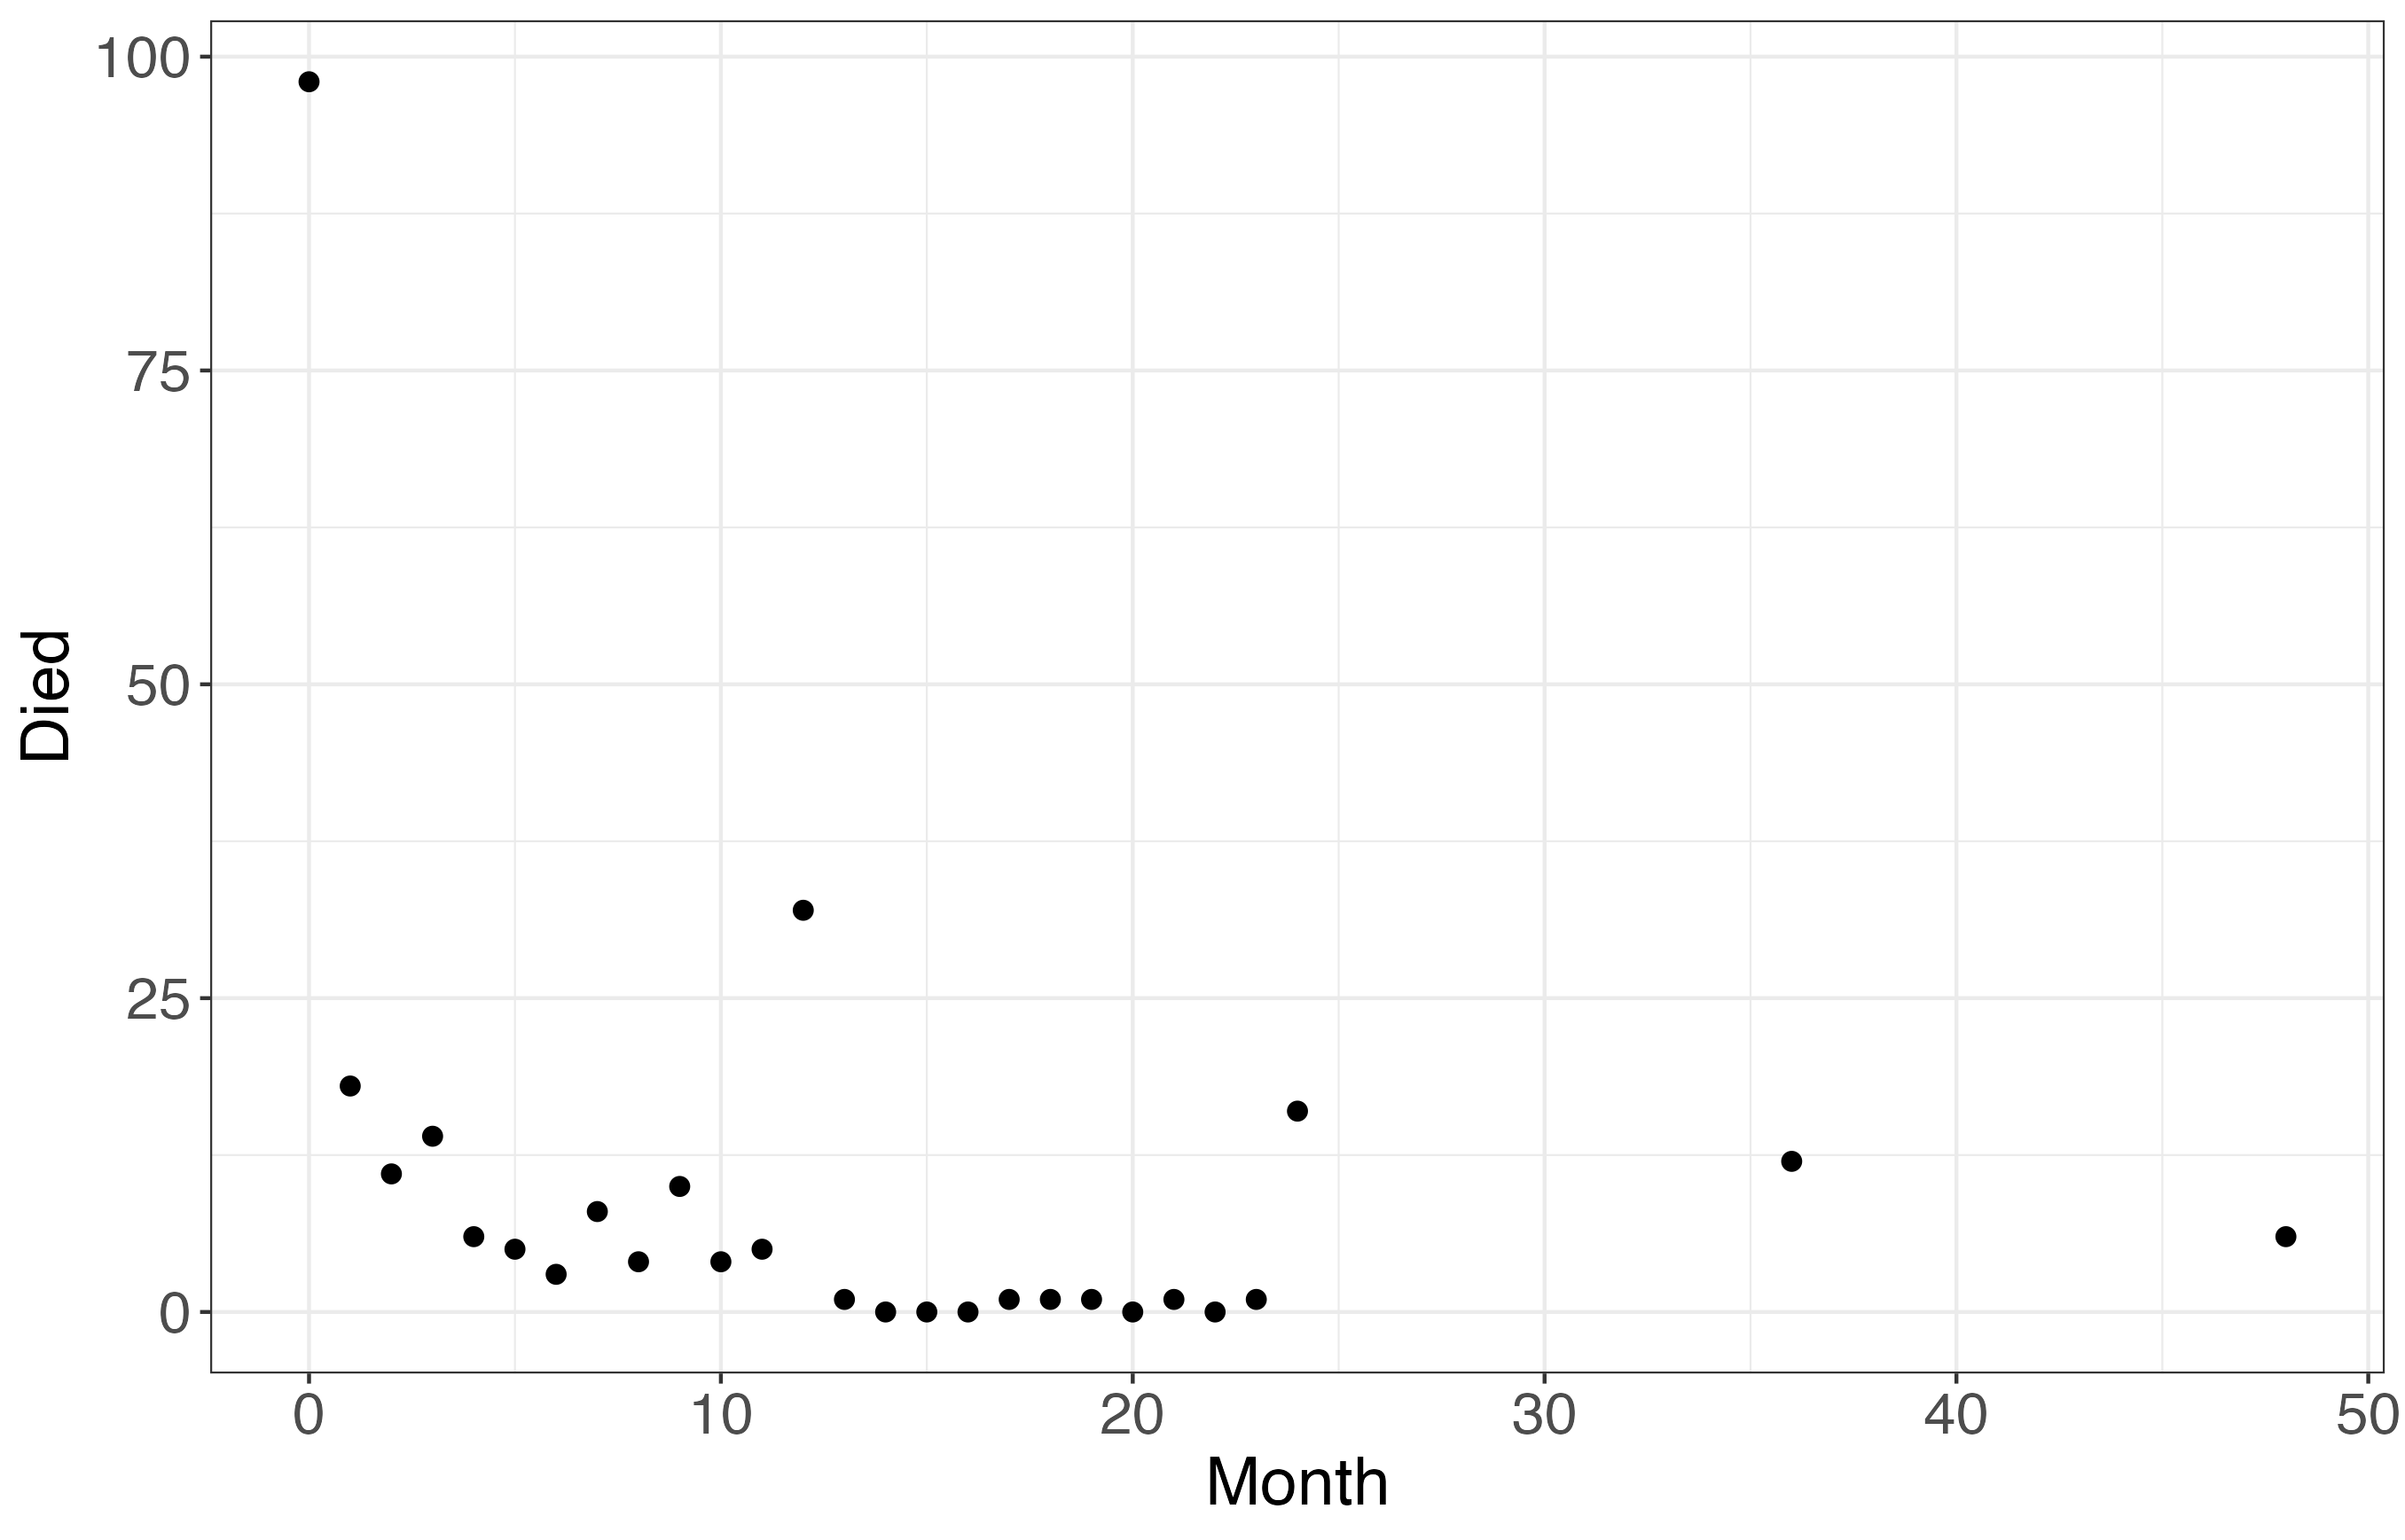
\includegraphics{u5mr.png}
\end{frame}

\begin{frame}{Types of Variables: Activity}
\protect\hypertarget{types-of-variables-activity-2}{}
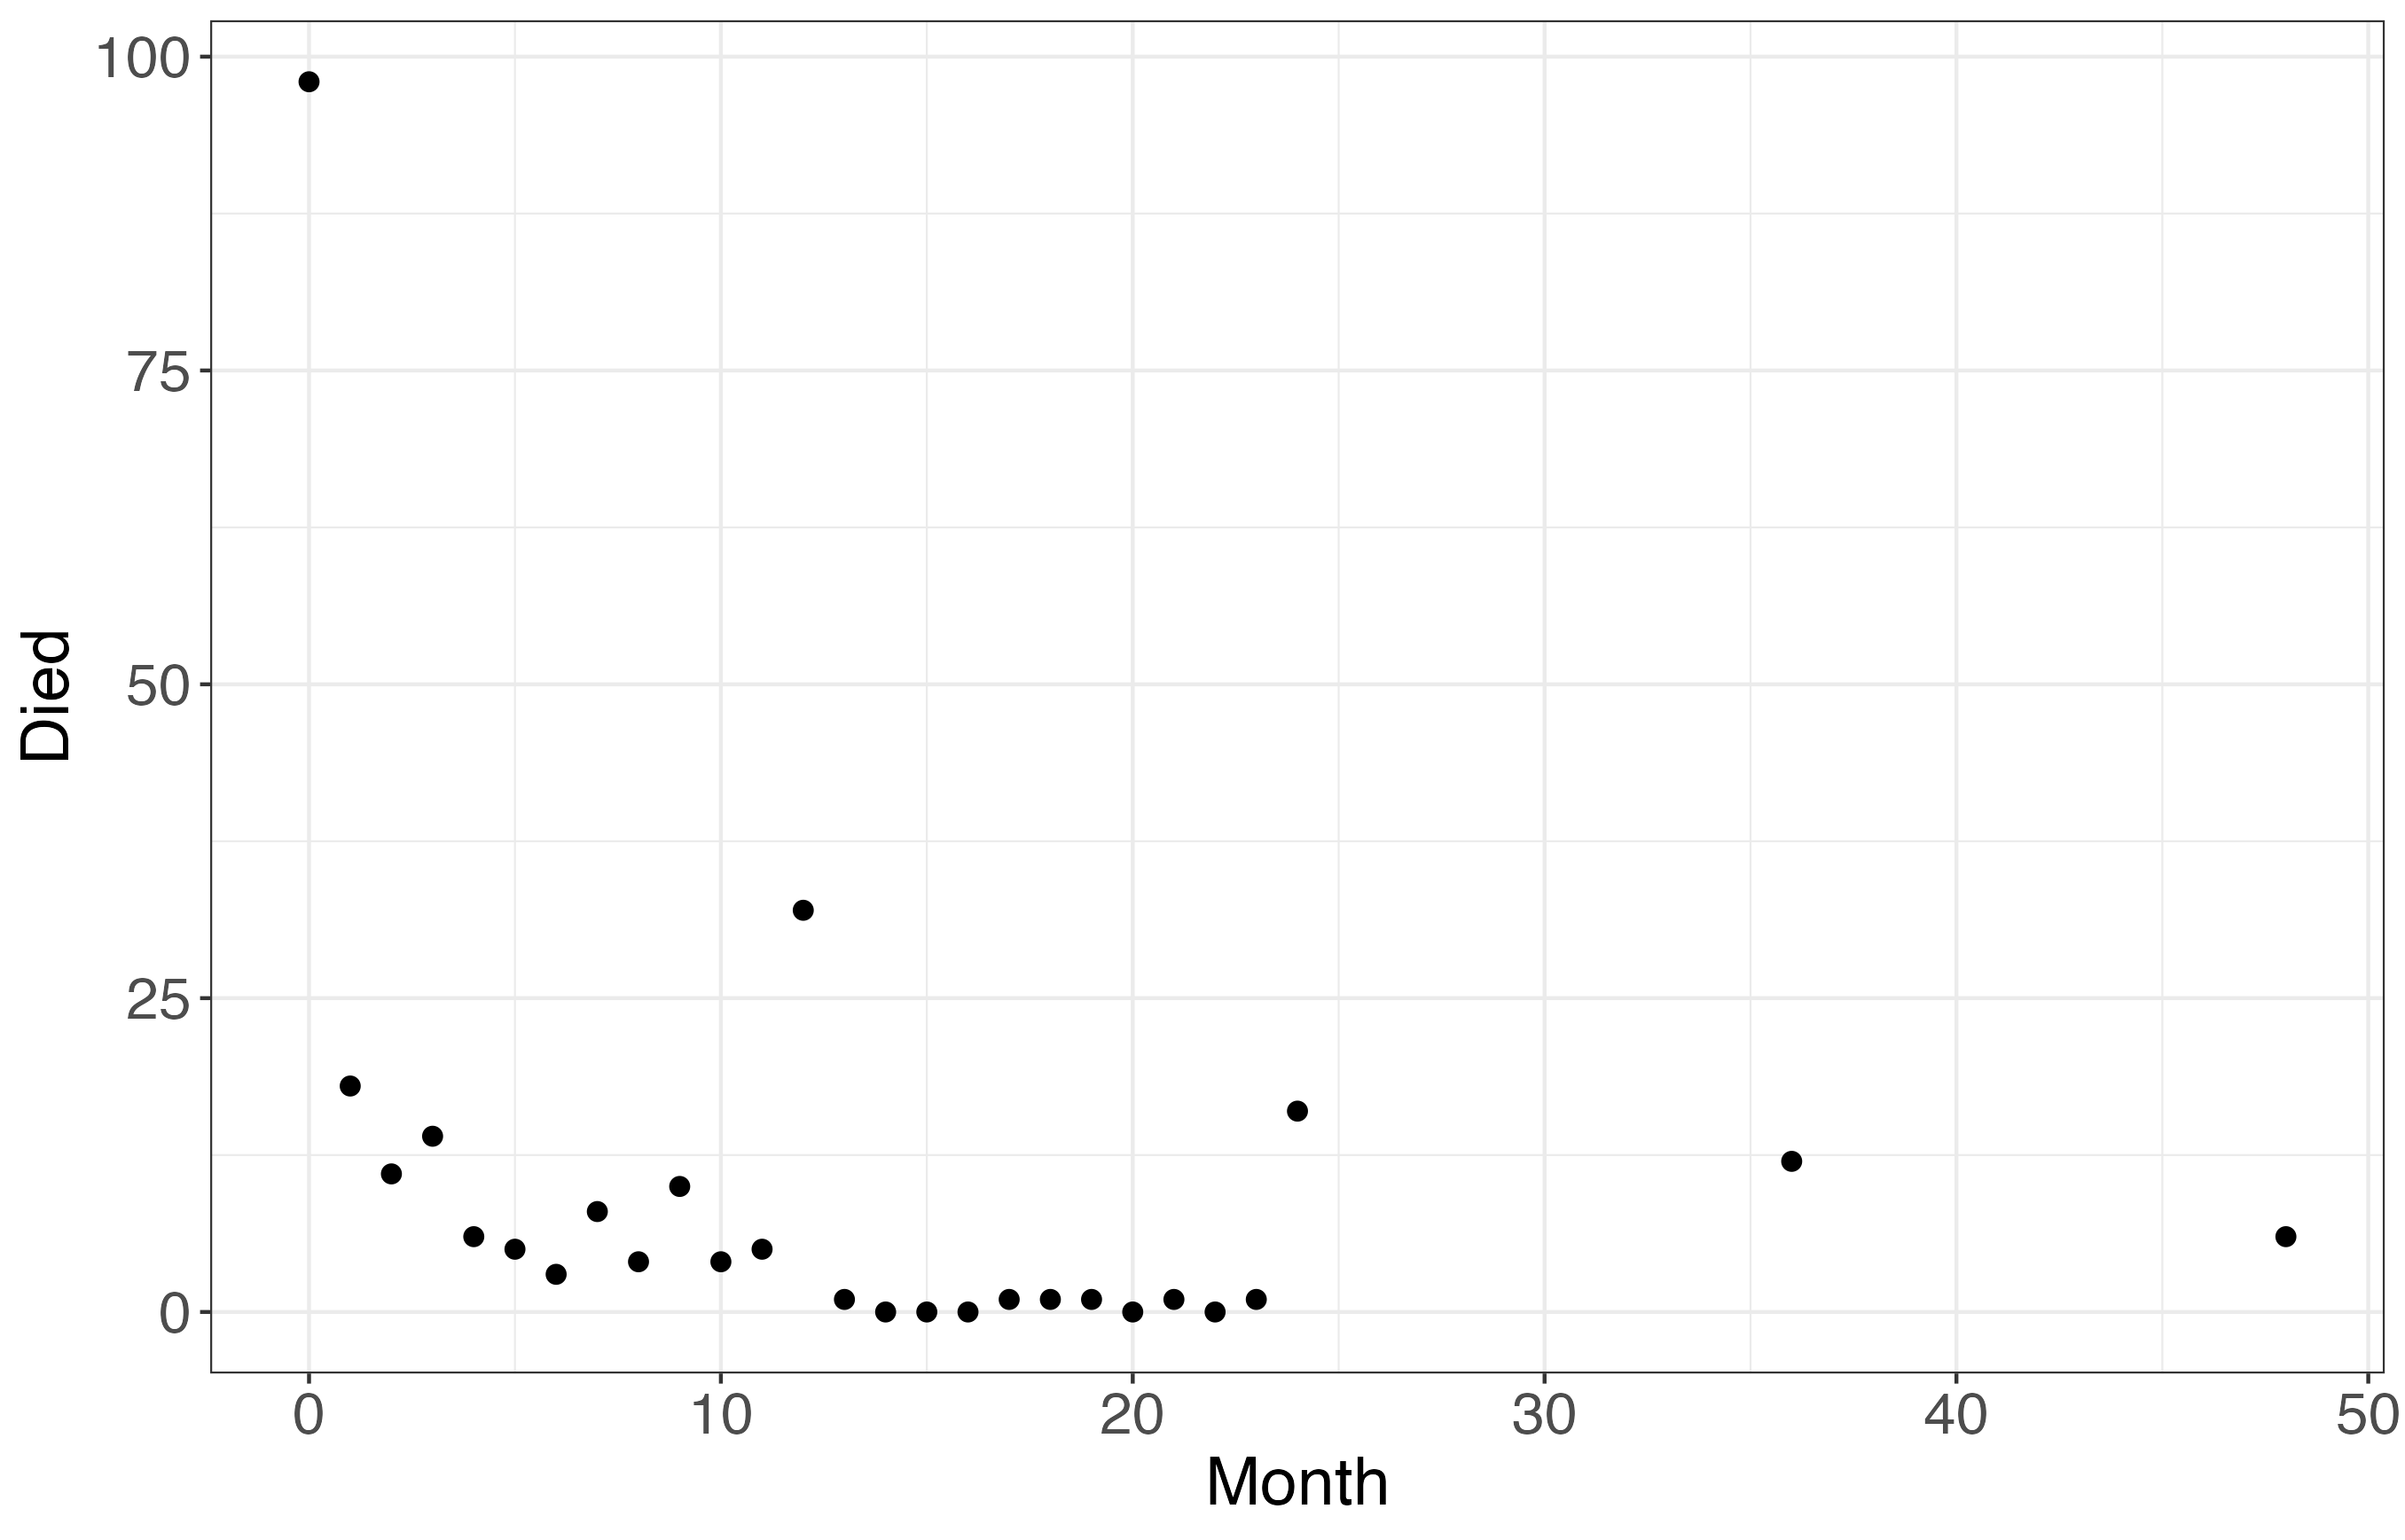
\includegraphics{u5mr.png}

\begin{itemize}
\tightlist
\item
  Argue why we should consider age at death to be a continuous variable.
\item
  Argue why we should consider age at death to be a discrete variable.
\item
  Do you notice anything strange about the plot? Does this affect
  whether or not we should consider age at death to be continuous or
  discrete?
\end{itemize}
\end{frame}

\begin{frame}{Types of Variables: Activity}
\protect\hypertarget{types-of-variables-activity-3}{}
Argue why we should consider age at death to be a continuous variable.

\begin{itemize}
\tightlist
\item
  {Age} is inherently continuous. We could, in theory, have ages
  recorded with an infinite number of decimal points.
\end{itemize}

Argue why we should consider age at death to be a discrete variable.

\begin{itemize}
\tightlist
\item
  {Age} is collected discretely in the survey. According to the survey,
  children could not be 2.5 years old, for example.
\end{itemize}
\end{frame}

\begin{frame}{Types of Variables: Activity}
\protect\hypertarget{types-of-variables-activity-4}{}
Do you notice anything strange about the plot? Does this affect whether
or not we should consider age at death to be continuous or discrete?

\begin{itemize}
\item
  {Death} counts seem to be higher at exact years than for the months in
  between 1-2 years. For 24 months, 3 years, and 4 years, this is likely
  due to grouping. If a child died between ages 2.5 - 3.5, they would be
  recorded as having died at 3 years, so this count would be inherently
  higher since it spans a longer time period than simply 1 month.
  However, what about 12 months?
\item
  {This phenomenon is known as ``age-heaping''}, and often occurs in
  surveys where parents do not know the exact age their child was when
  they died, or when surveyers themselves record dates inexactly. This
  is essentially a rounding error, where many deaths are recorded at 1
  year even though they may have occurred at any time between 0 and 2
  years.
\end{itemize}
\end{frame}

\begin{frame}{Types of Variables: Activity}
\protect\hypertarget{types-of-variables-activity-5}{}
Considering age to be continuous \emph{or} discrete in this example are
both justifiable conclusions! In general, we'll consider age to be
continuous in this class, but in specific scenarios it may make more
sense to consider age in discrete groups.
\end{frame}

\begin{frame}{Descriptive statistics vs.~Inferential statistics}
\protect\hypertarget{descriptive-statistics-vs.-inferential-statistics}{}
Some terms you should know:

\begin{itemize}
\tightlist
\item
  {Descriptive statistics}: summarize or {describe} what's happening
  {\textbf{in our sample}}\\
\item
  {Inferential statistics}: use our data to {infer} something about
  {\textbf{our population of interest}}
\end{itemize}

Often when people talk about ``doing statistics,'' they're talking about
inferential statistics.

But statistics is much more than that. In fact, \textbf{the most
important part of statistics (and often the hardest) }is translating
your scientific question into a statistics question. Once you've done
this, the rest follows.
\end{frame}

\begin{frame}{Descriptive Statistics}
\protect\hypertarget{descriptive-statistics}{}
Why do we need descriptive statistics?

\begin{itemize}
\item
  Making sense of large amounts of data
\item
  Checking data quality
\item
  Values outside reasonable range (e.g., height = 9')
\item
  Implausible combinations of variables (e.g., positive test for
  cervical cancer for a person without a cervix)
\item
  Observe distribution of variables in dataset
\item
  Measures of center and spread
\item
  Start to understand direction and strength of association
\item
  Descriptive statistics and inferential statistics should contribute to
  the same story
\end{itemize}
\end{frame}

\begin{frame}{Descriptive Statistics}
\protect\hypertarget{descriptive-statistics-1}{}
Appropriate descriptive statistics will vary depending on what how many
variables you want to describe at once, and whether or not you want
numerical or graphical summaries.

Outline:

\begin{itemize}
\item
  Univariate

  \begin{itemize}
  \tightlist
  \item
    Numerical (categorical variables)
  \item
    Numerical (quantitative variables)
  \end{itemize}
\item
  Stratified/Bivariate

  \begin{itemize}
  \tightlist
  \item
    Numerical summaries, broken down by group
  \item
    Graphical
  \end{itemize}
\end{itemize}
\end{frame}

\begin{frame}{Univariate Descriptive Statistics: Categorical}
\protect\hypertarget{univariate-descriptive-statistics-categorical}{}
{Example}: In our births dataset, we have an indicator variable for
whether or not an individual particpated in the First Steps program or
not.

Suppose we are interested in knowing how many individuals fall into each
group. How would we summarize this data?
\end{frame}

\begin{frame}{Univariate Descriptive Statistics: Categorical}
\protect\hypertarget{univariate-descriptive-statistics-categorical-1}{}
We could begin by counting up the number of individuals that fall in
each category:

\begin{longtable}[]{@{}ll@{}}
\toprule
\textbf{First Steps participation} & \textbf{Number of Individuals} \\
\midrule
\endhead
Yes & 403 \\
No & 2097 \\
\bottomrule
\end{longtable}

Note that no one in our dataset had a missing value for First Steps
participation. If we did have any missing values, we could include this
information as an additional ``NA'' row in our table
\end{frame}

\begin{frame}{Univariate Descriptive Statistics: Categorical}
\protect\hypertarget{univariate-descriptive-statistics-categorical-2}{}
We can also report the proportion of individuals that fall in each
group:

\begin{longtable}[]{@{}ll@{}}
\toprule
\textbf{First Steps participation} & \textbf{Proportion of Individuals
(No.)} \\
\midrule
\endhead
Yes & 16.1\% (403) \\
No & 83.9\% (2097) \\
\bottomrule
\end{longtable}
\end{frame}

\begin{frame}{Univariate Descriptive Statistics: Categorical}
\protect\hypertarget{univariate-descriptive-statistics-categorical-3}{}
Summary should include:

\begin{itemize}
\item
  Number and percent in each group
\item
  If binary, only need to summarize one group
\item
  The other can be inferred (for example, we had 16.1 \% of individuals
  participate in First Steps, so 100 - 16.1 = 83.9 \% did not.)
\item
  Also good to summarize missing data

  \begin{itemize}
  \tightlist
  \item
    e.g., \# and proportion of missing values
  \end{itemize}
\end{itemize}
\end{frame}

\begin{frame}{Univariate Desc. Stats.: Quantitative}
\protect\hypertarget{univariate-desc.-stats.-quantitative}{}
{Example}: The primary outcome of interest in our births dataset is
birthweight, recorded in grams. The data for birthweight:

\begin{longtable}[]{@{}ll@{}}
\toprule
\textbf{Individual ID} & \textbf{Birthweight (grams)} \\
\midrule
\endhead
1 & 3118 \\
2 & 3466 \\
3 & 3147 \\
\ldots{} & \ldots{} \\
2498 & 3005 \\
2499 & 1644 \\
2500 & 3317 \\
\bottomrule
\end{longtable}

What information may be useful to know?
\end{frame}

\begin{frame}{Univariate Descriptive Statistics: Quantitative}
\protect\hypertarget{univariate-descriptive-statistics-quantitative}{}
How many individuals are in our dataset?

\begin{itemize}
\tightlist
\item
  {[}{]} {There are 2500 individuals in our dataset.}
\end{itemize}

Do any individuals have missing values for birthweight?

\begin{itemize}
\tightlist
\item
  {[}{]} {No!}
\end{itemize}

Measures of center?

\begin{itemize}
\tightlist
\item
  {Mean birthweight is 3414} grams.
\item
  {Median birthweight is 3444 grams.}
\end{itemize}

Measures of spread?

\begin{itemize}
\tightlist
\item
  {Sample standard deviation is 559 grams.}
\item
  {Interquartile range (IQR) is (3096 grams, 3766 grams) (Q1, Q3) }
\item
  {Range is (255 grams, 5175 grams)} (The smallest baby to ever survive
  weighed around 212 grams)
\end{itemize}
\end{frame}

\begin{frame}{Univariate Descriptive Statistics: Quantitative}
\protect\hypertarget{univariate-descriptive-statistics-quantitative-1}{}
Summary should include (some of):

\begin{itemize}
\item
  Sample size / number of observations
\item
  Number of missing observations
\item
  Measures of center:
\item
  Sample mean
\item
  Sample median
\item
  Measures of spread:
\item
  Sample standard deviation
\item
  Interquartile range (IQR): (Q1, Q3) or (Q3 - Q1)
\item
  Range: (Min, Max) or (Max - Min)
\end{itemize}
\end{frame}

\begin{frame}{Univariate Descriptive Statistics: Graphical}
\protect\hypertarget{univariate-descriptive-statistics-graphical}{}
For categorical variables, we can make barplots:

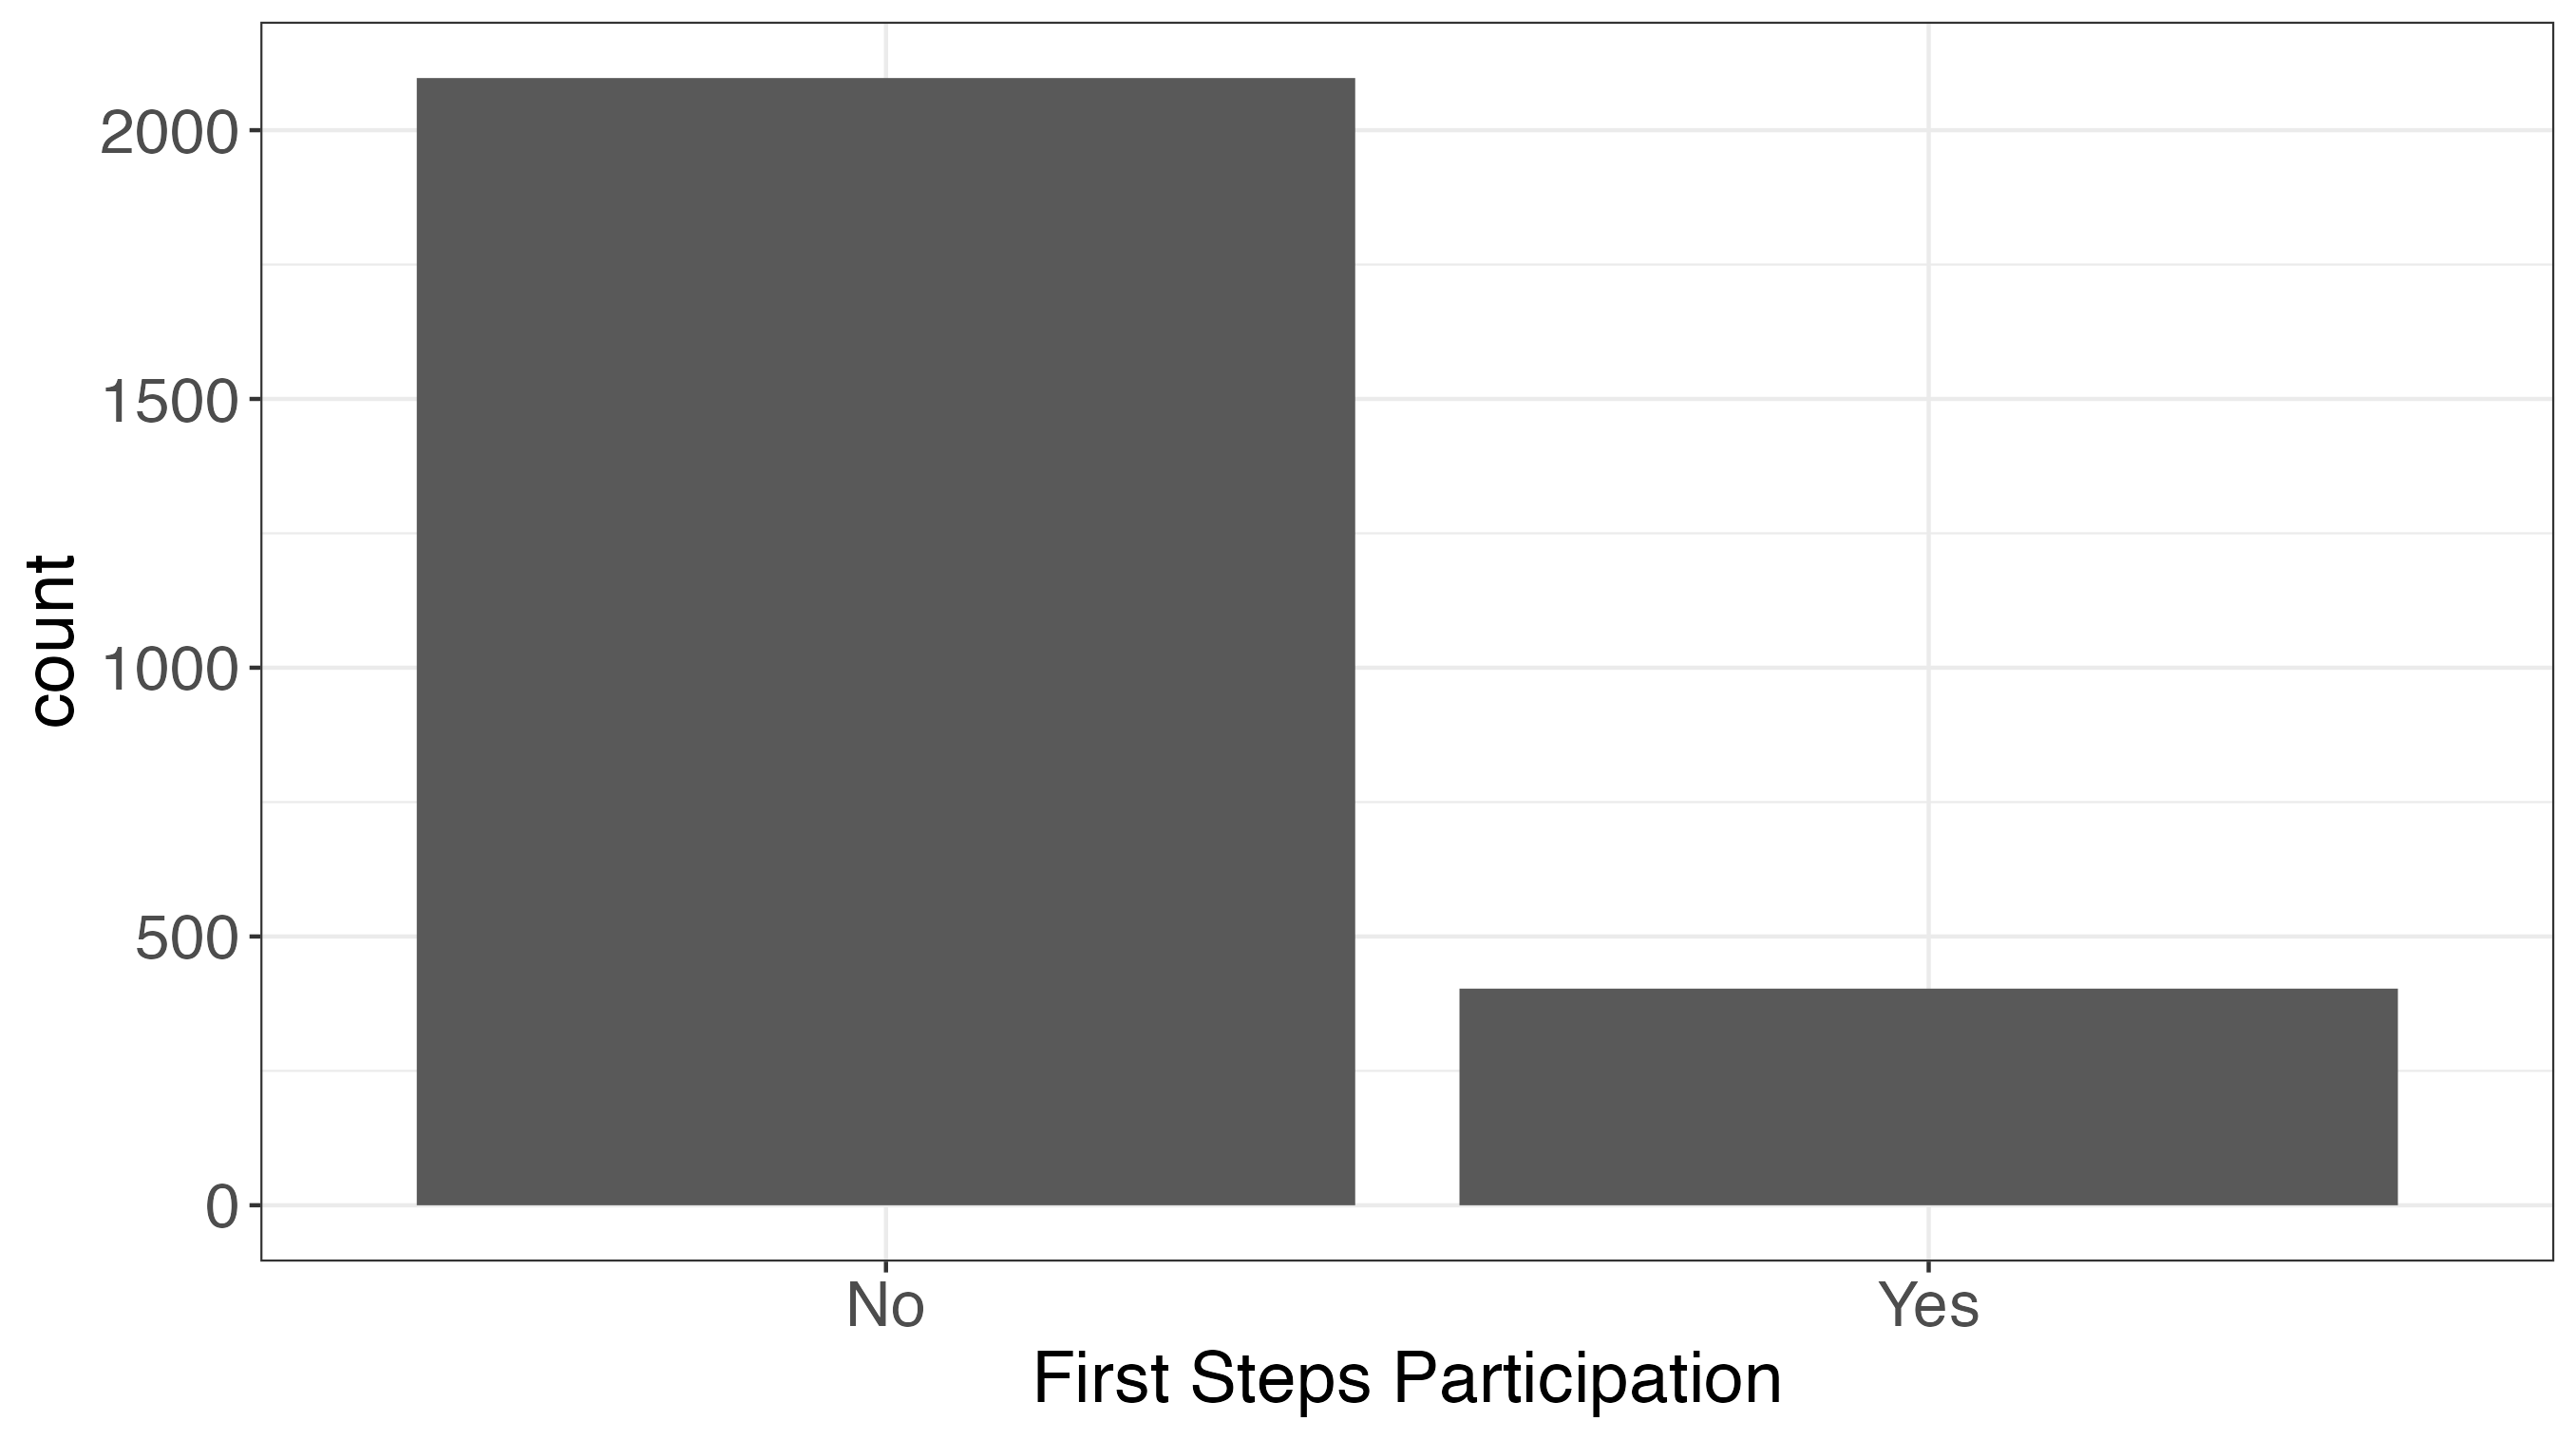
\includegraphics{fs_bar.png}
\end{frame}

\begin{frame}{Univariate Descriptive Statistics: Graphical}
\protect\hypertarget{univariate-descriptive-statistics-graphical-1}{}
For quantitative variables, we can make histograms and boxplots.
Histograms are useful for describing the shape of the distribution of a
variable, and boxplots are useful for seeing central tendency (and
sometimes outliers):

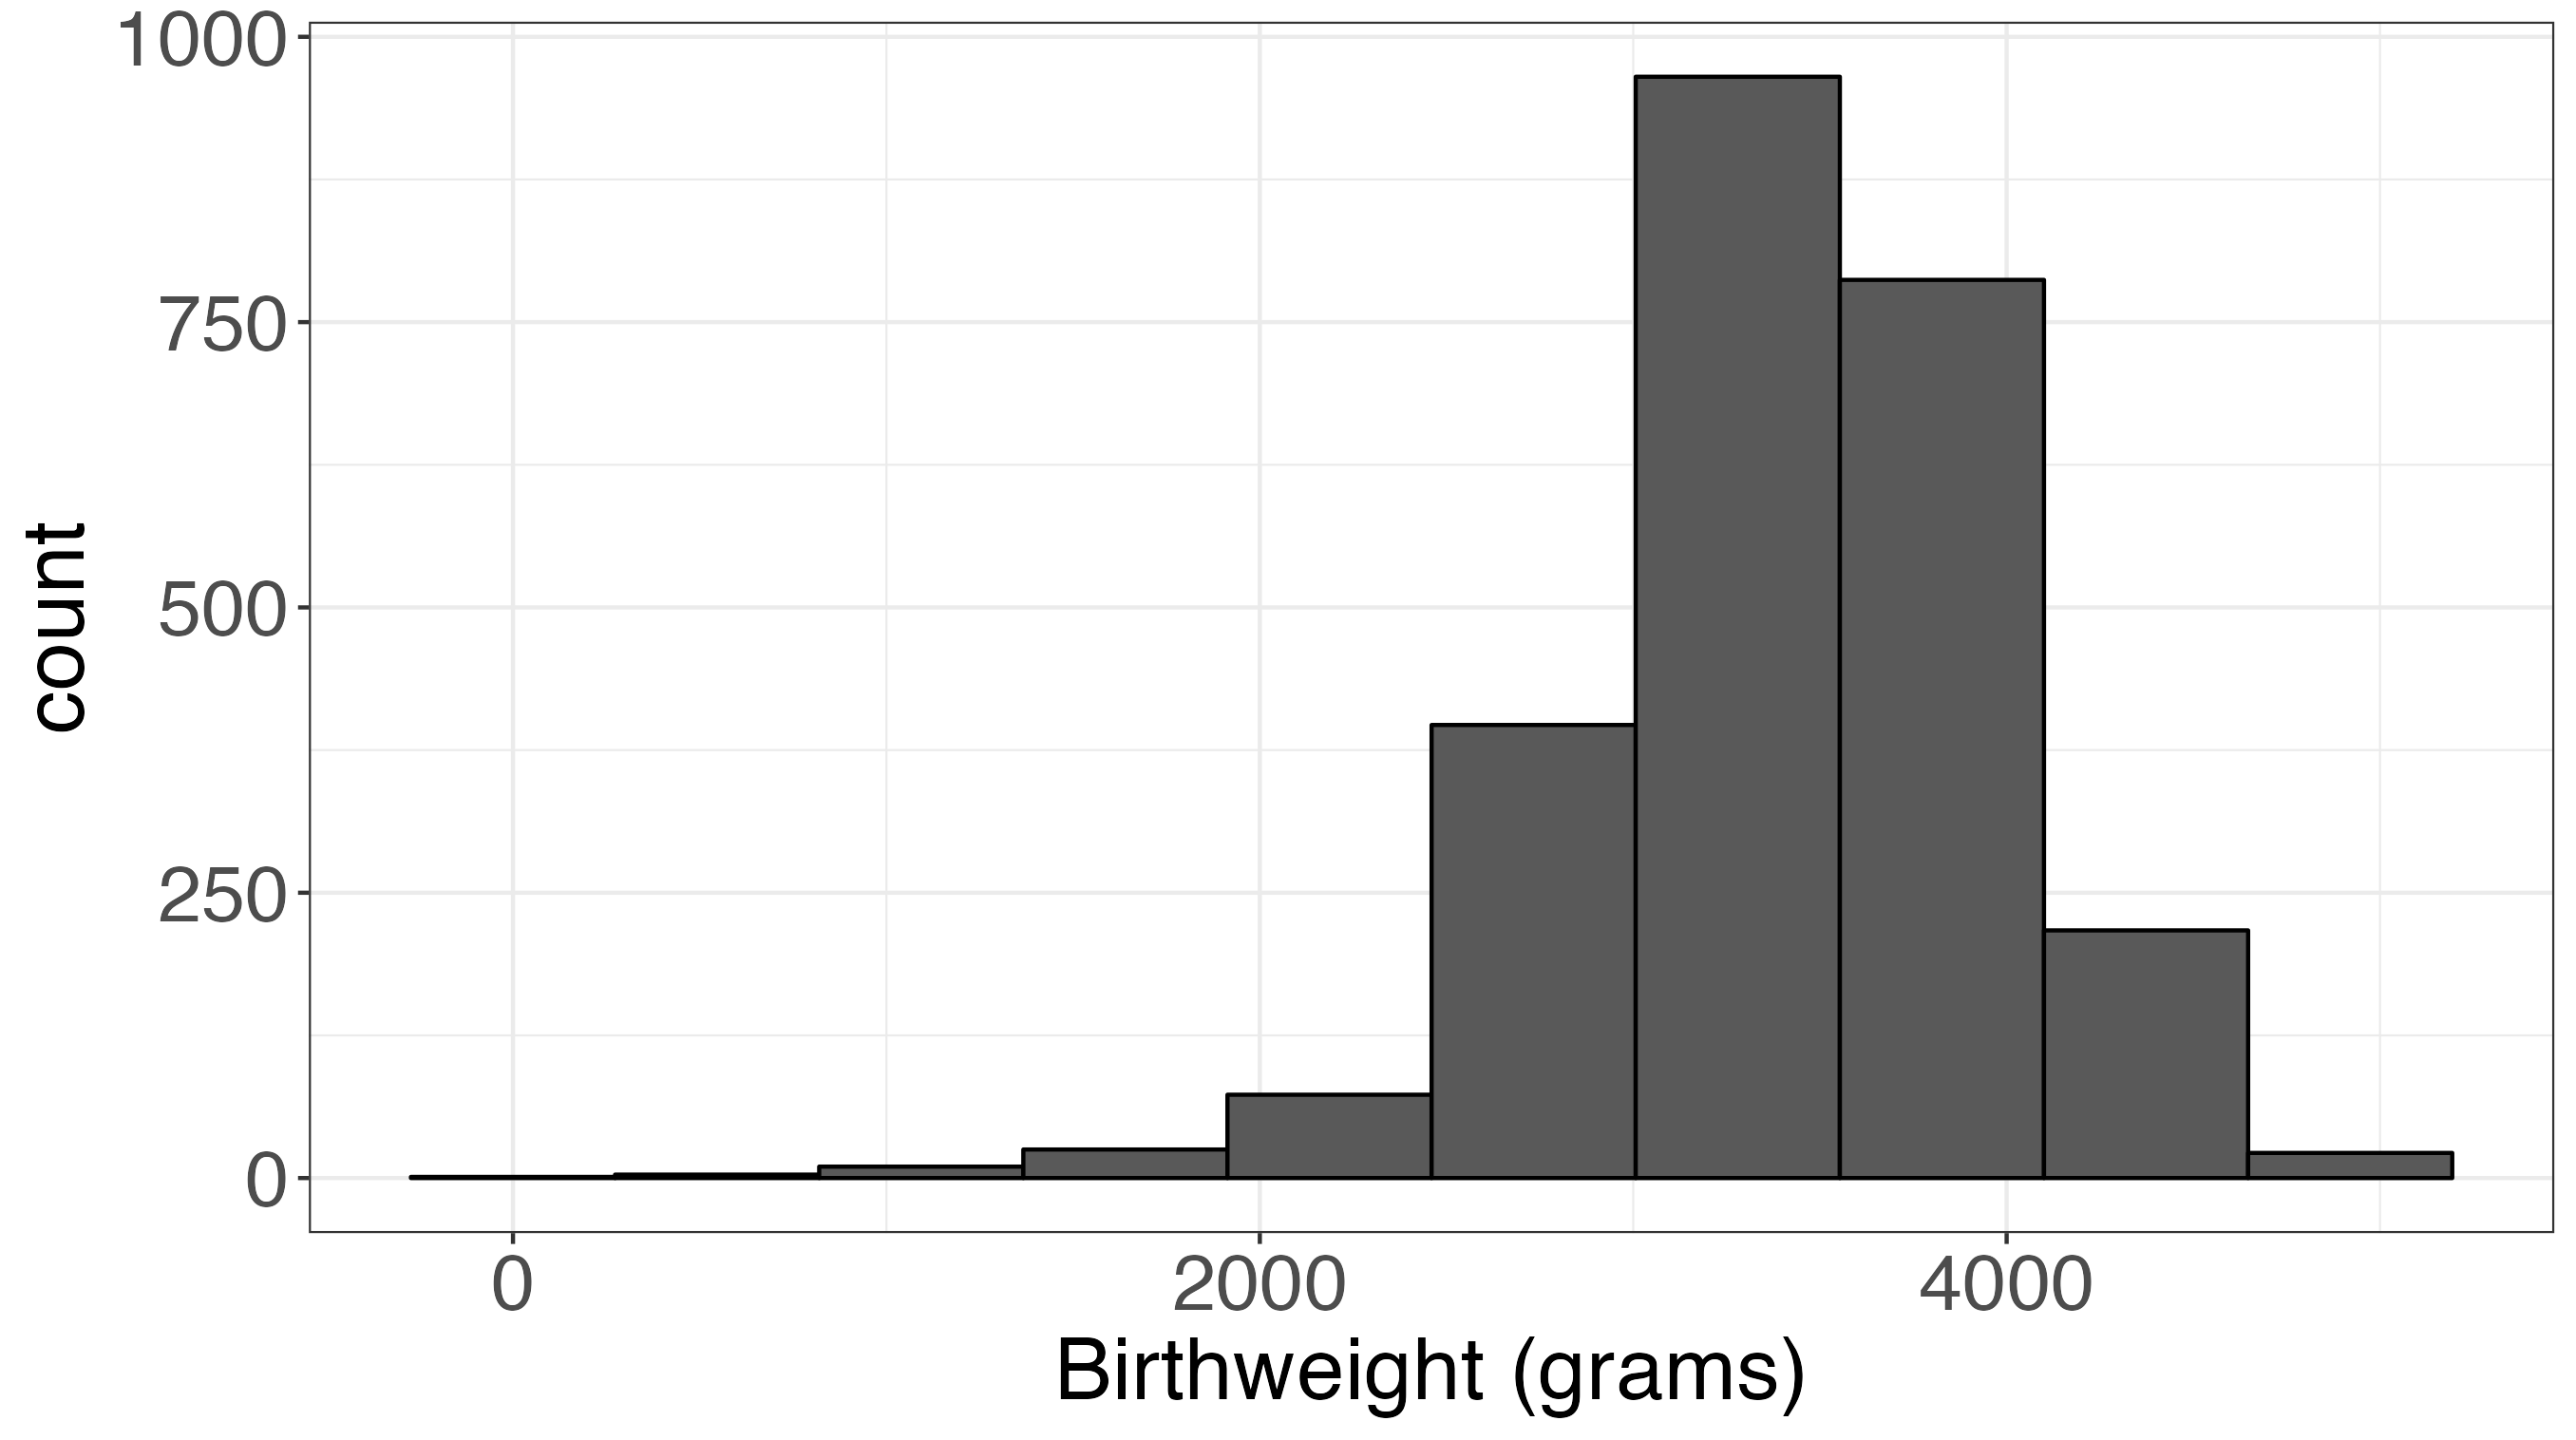
\includegraphics{fs_hist.png} 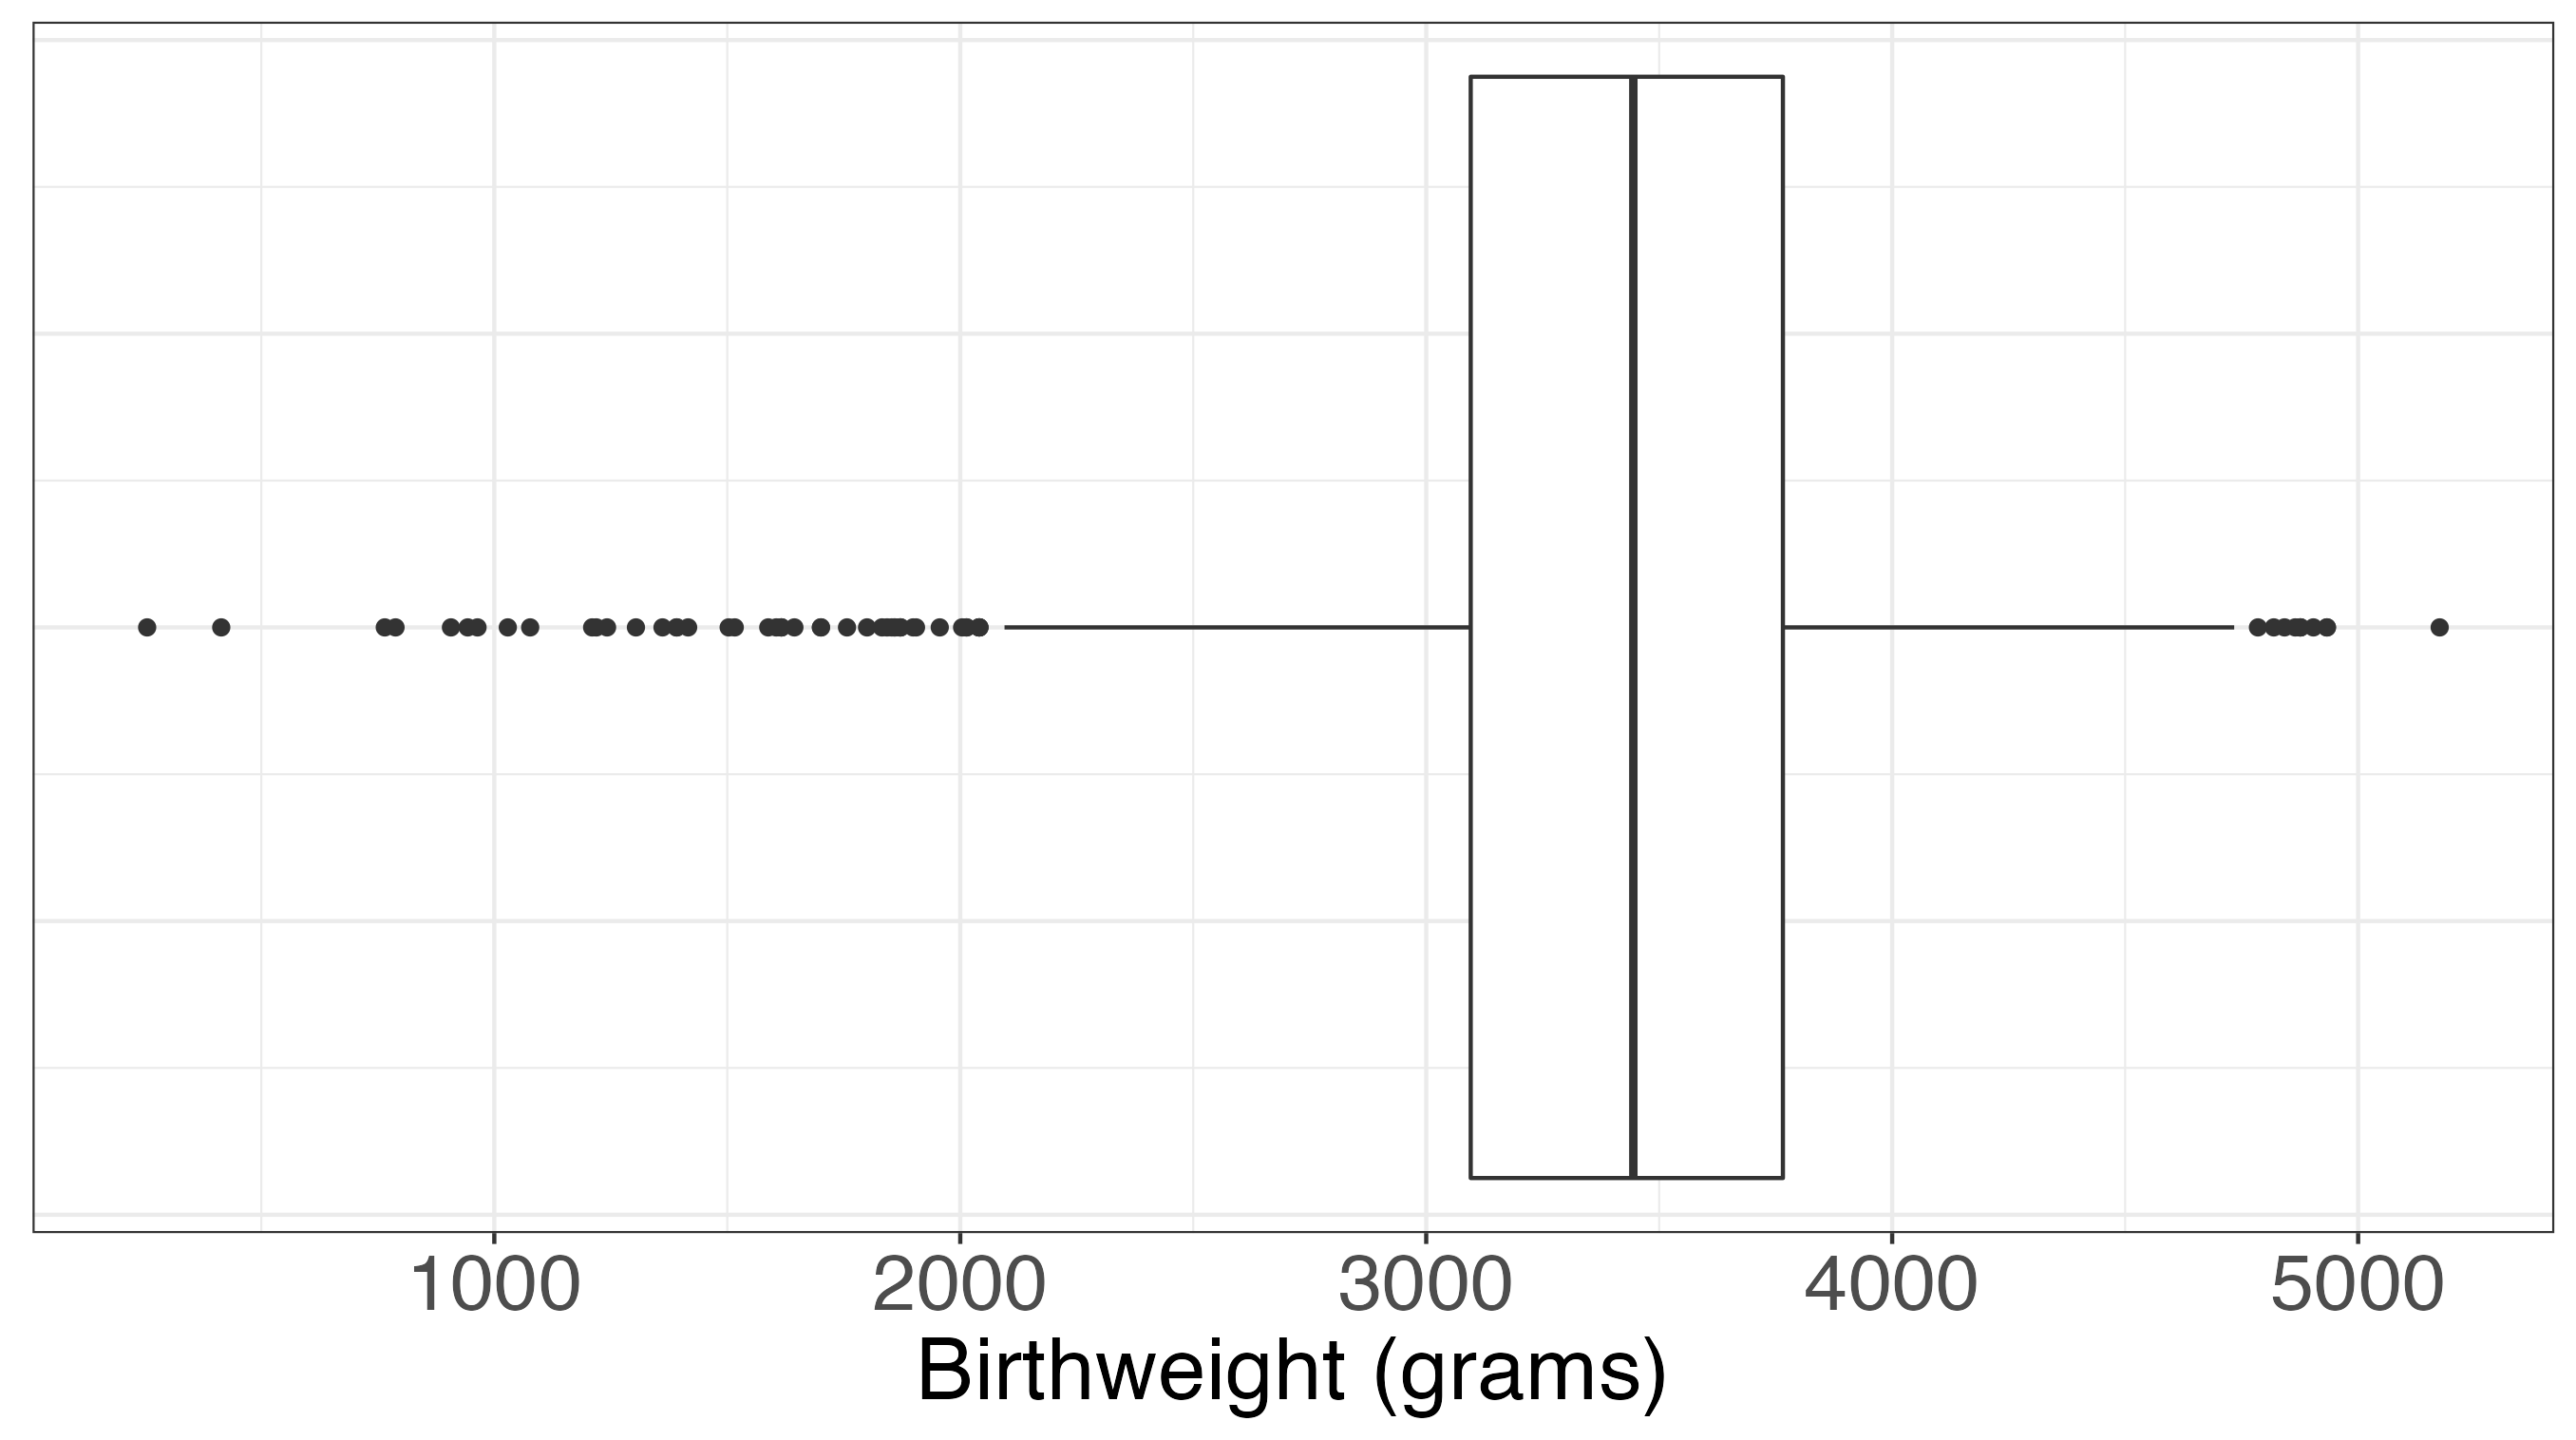
\includegraphics{fs_box.png}
\end{frame}

\begin{frame}{Stratified Descriptive Statistics: Graphical}
\protect\hypertarget{stratified-descriptive-statistics-graphical}{}
Sometimes we're interested in the distribution of a variable within
certain subgroups, rather than across all the data:

\begin{itemize}
\tightlist
\item
  e.g., how does the distribution of birthweights differ between
  individuals who pariticipated in First Steps and those who did not?
\end{itemize}

Stratified descriptive statistics can help us:

\begin{itemize}
\tightlist
\item
  Understand the role of the stratification variable
\item
  Begin to demonstrate the association between the two variables
\end{itemize}
\end{frame}

\begin{frame}{Stratified Descriptive Statistics: Graphical}
\protect\hypertarget{stratified-descriptive-statistics-graphical-1}{}
How does the distribution of birthweights differ between individuals who
participated in First Steps and those who did not? We can make
histograms for each category of individuals:

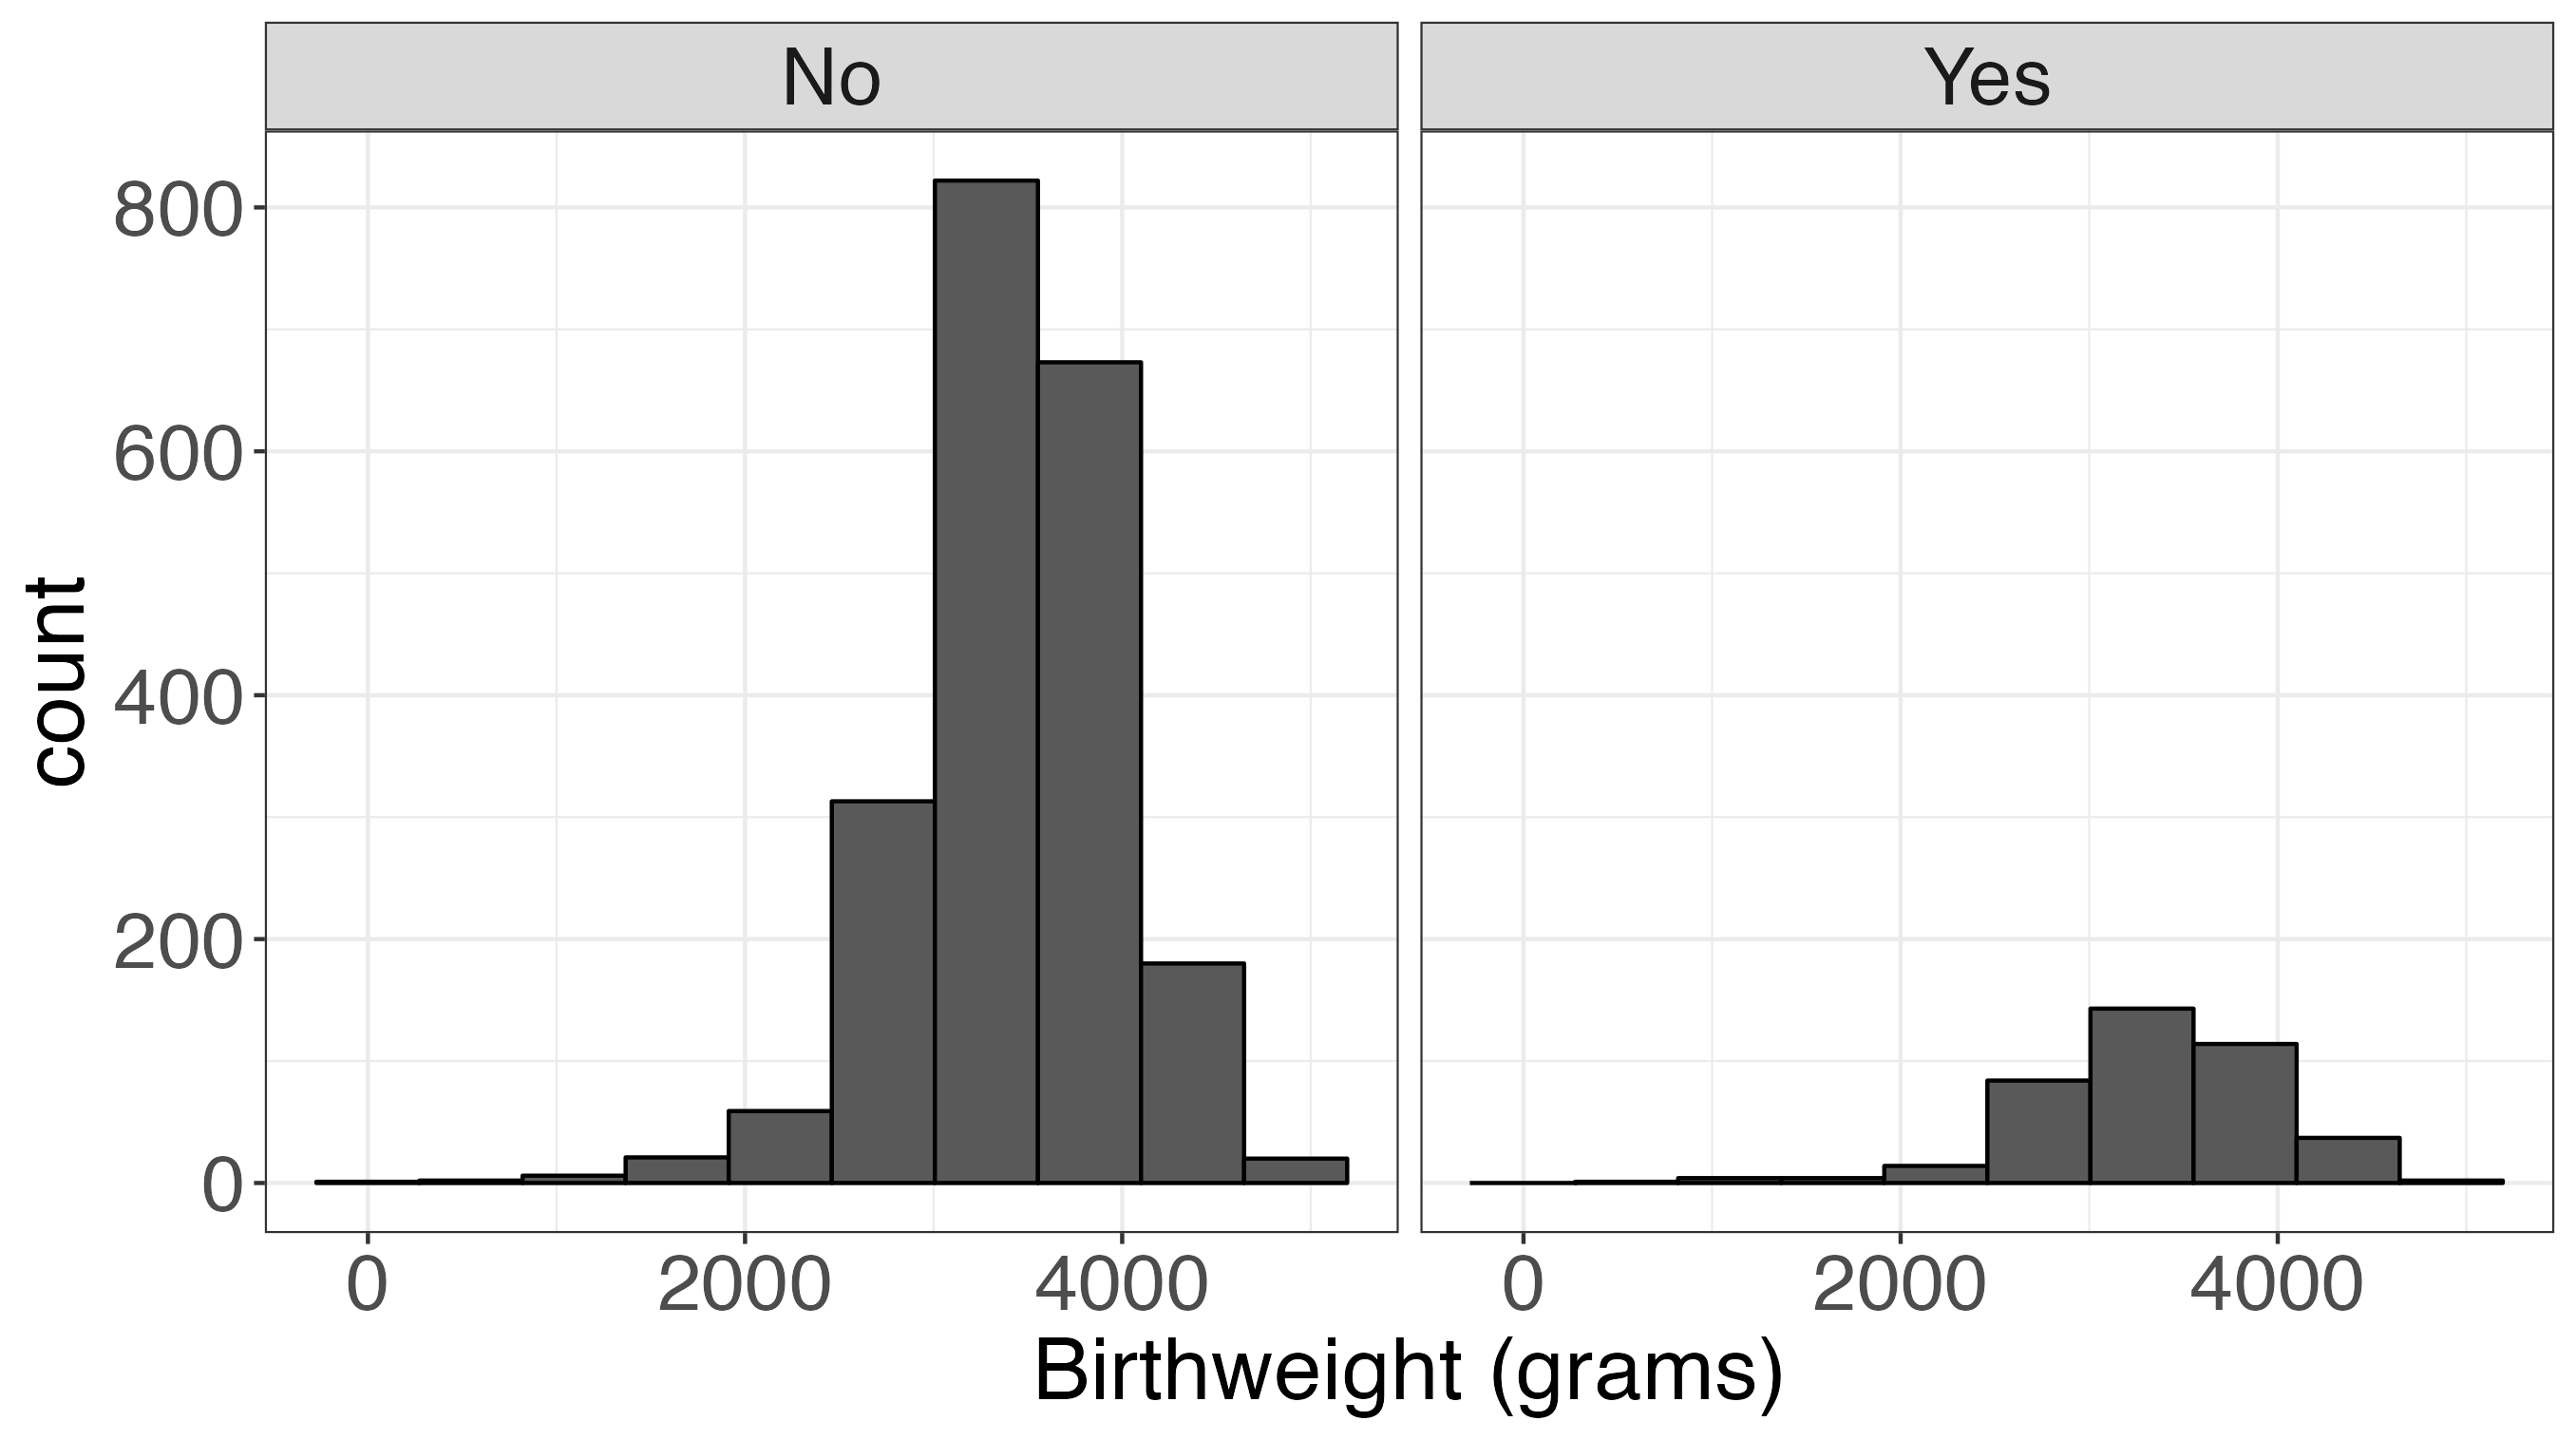
\includegraphics{fs_hist_firstep.png}
\end{frame}

\begin{frame}{Stratified Descriptive Statistics: Graphical}
\protect\hypertarget{stratified-descriptive-statistics-graphical-2}{}
We can also use side-by-side boxplots rather than side-by-side
histograms. It may be easier to see the median birthweight is slightly
lower in individuals who participated in First Steps:

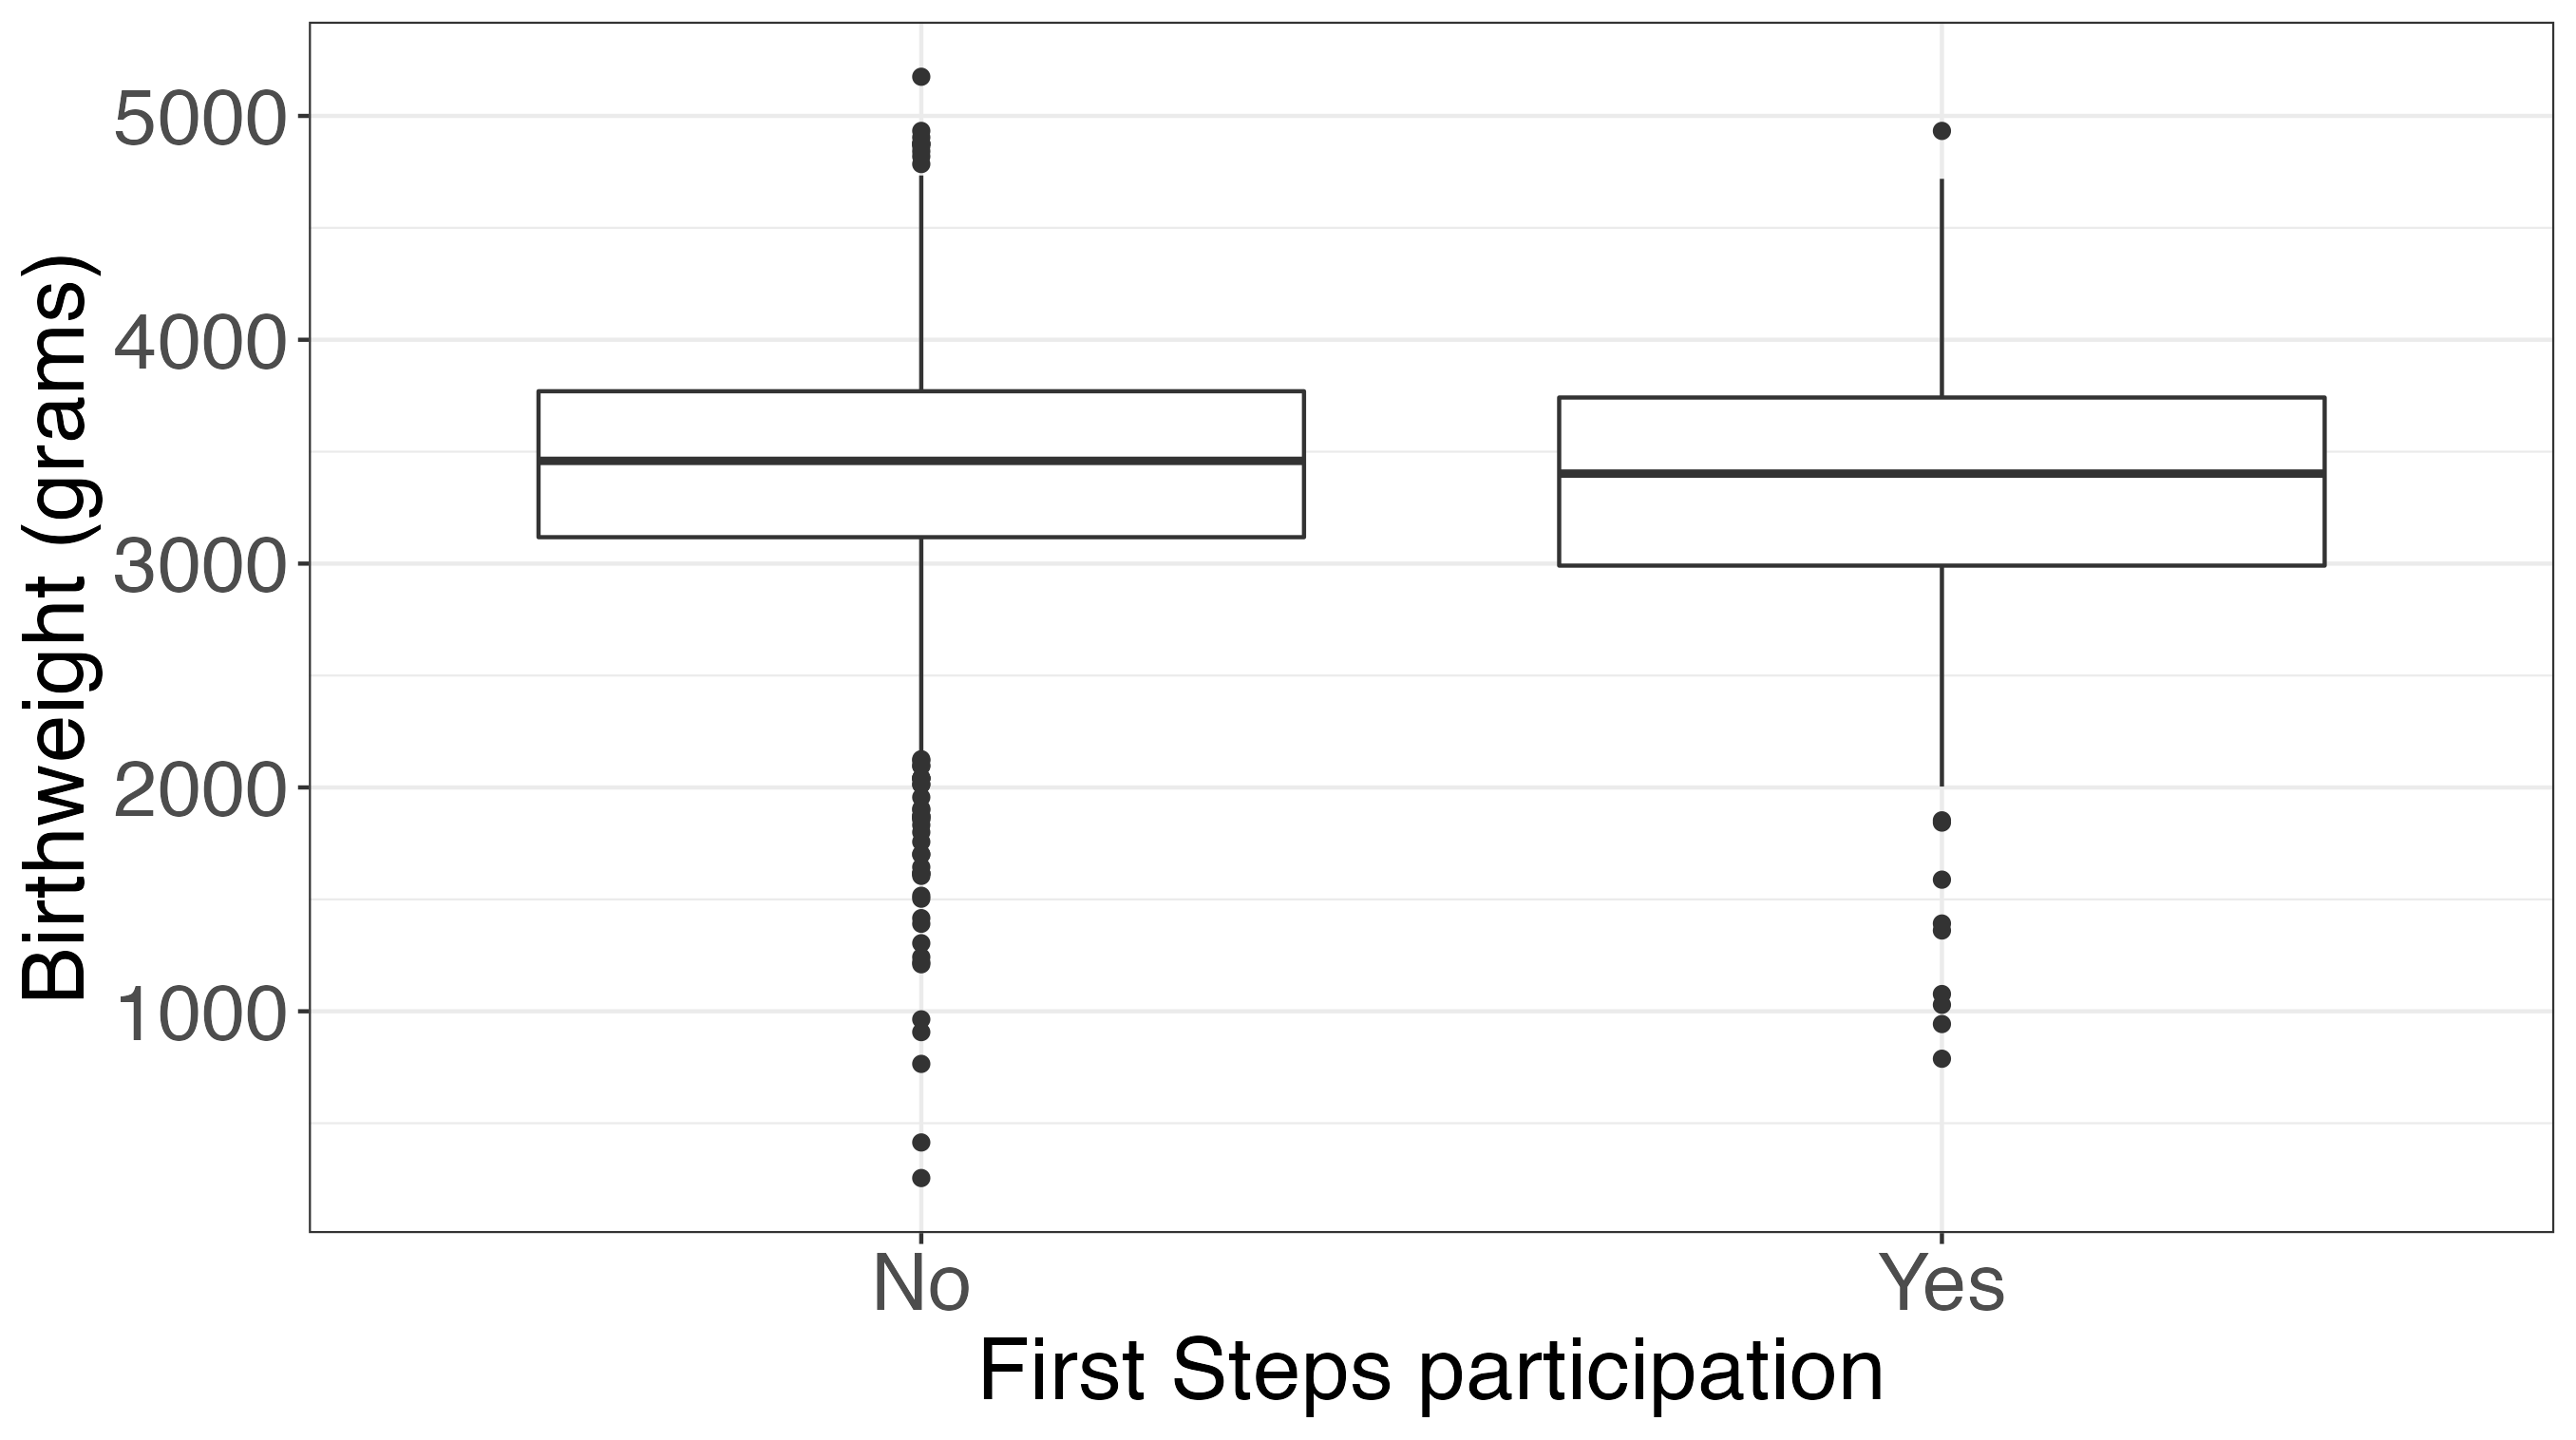
\includegraphics{fs_box_firstep.png}
\end{frame}

\begin{frame}{Stratified Descriptive Statistics: Graphical}
\protect\hypertarget{stratified-descriptive-statistics-graphical-3}{}
Scatterplots are a useful tool for summarizing the relationship between
two quantitative variables. Below we plot age in years vs.~birthweight
in grams for all individuals in our births dataset:

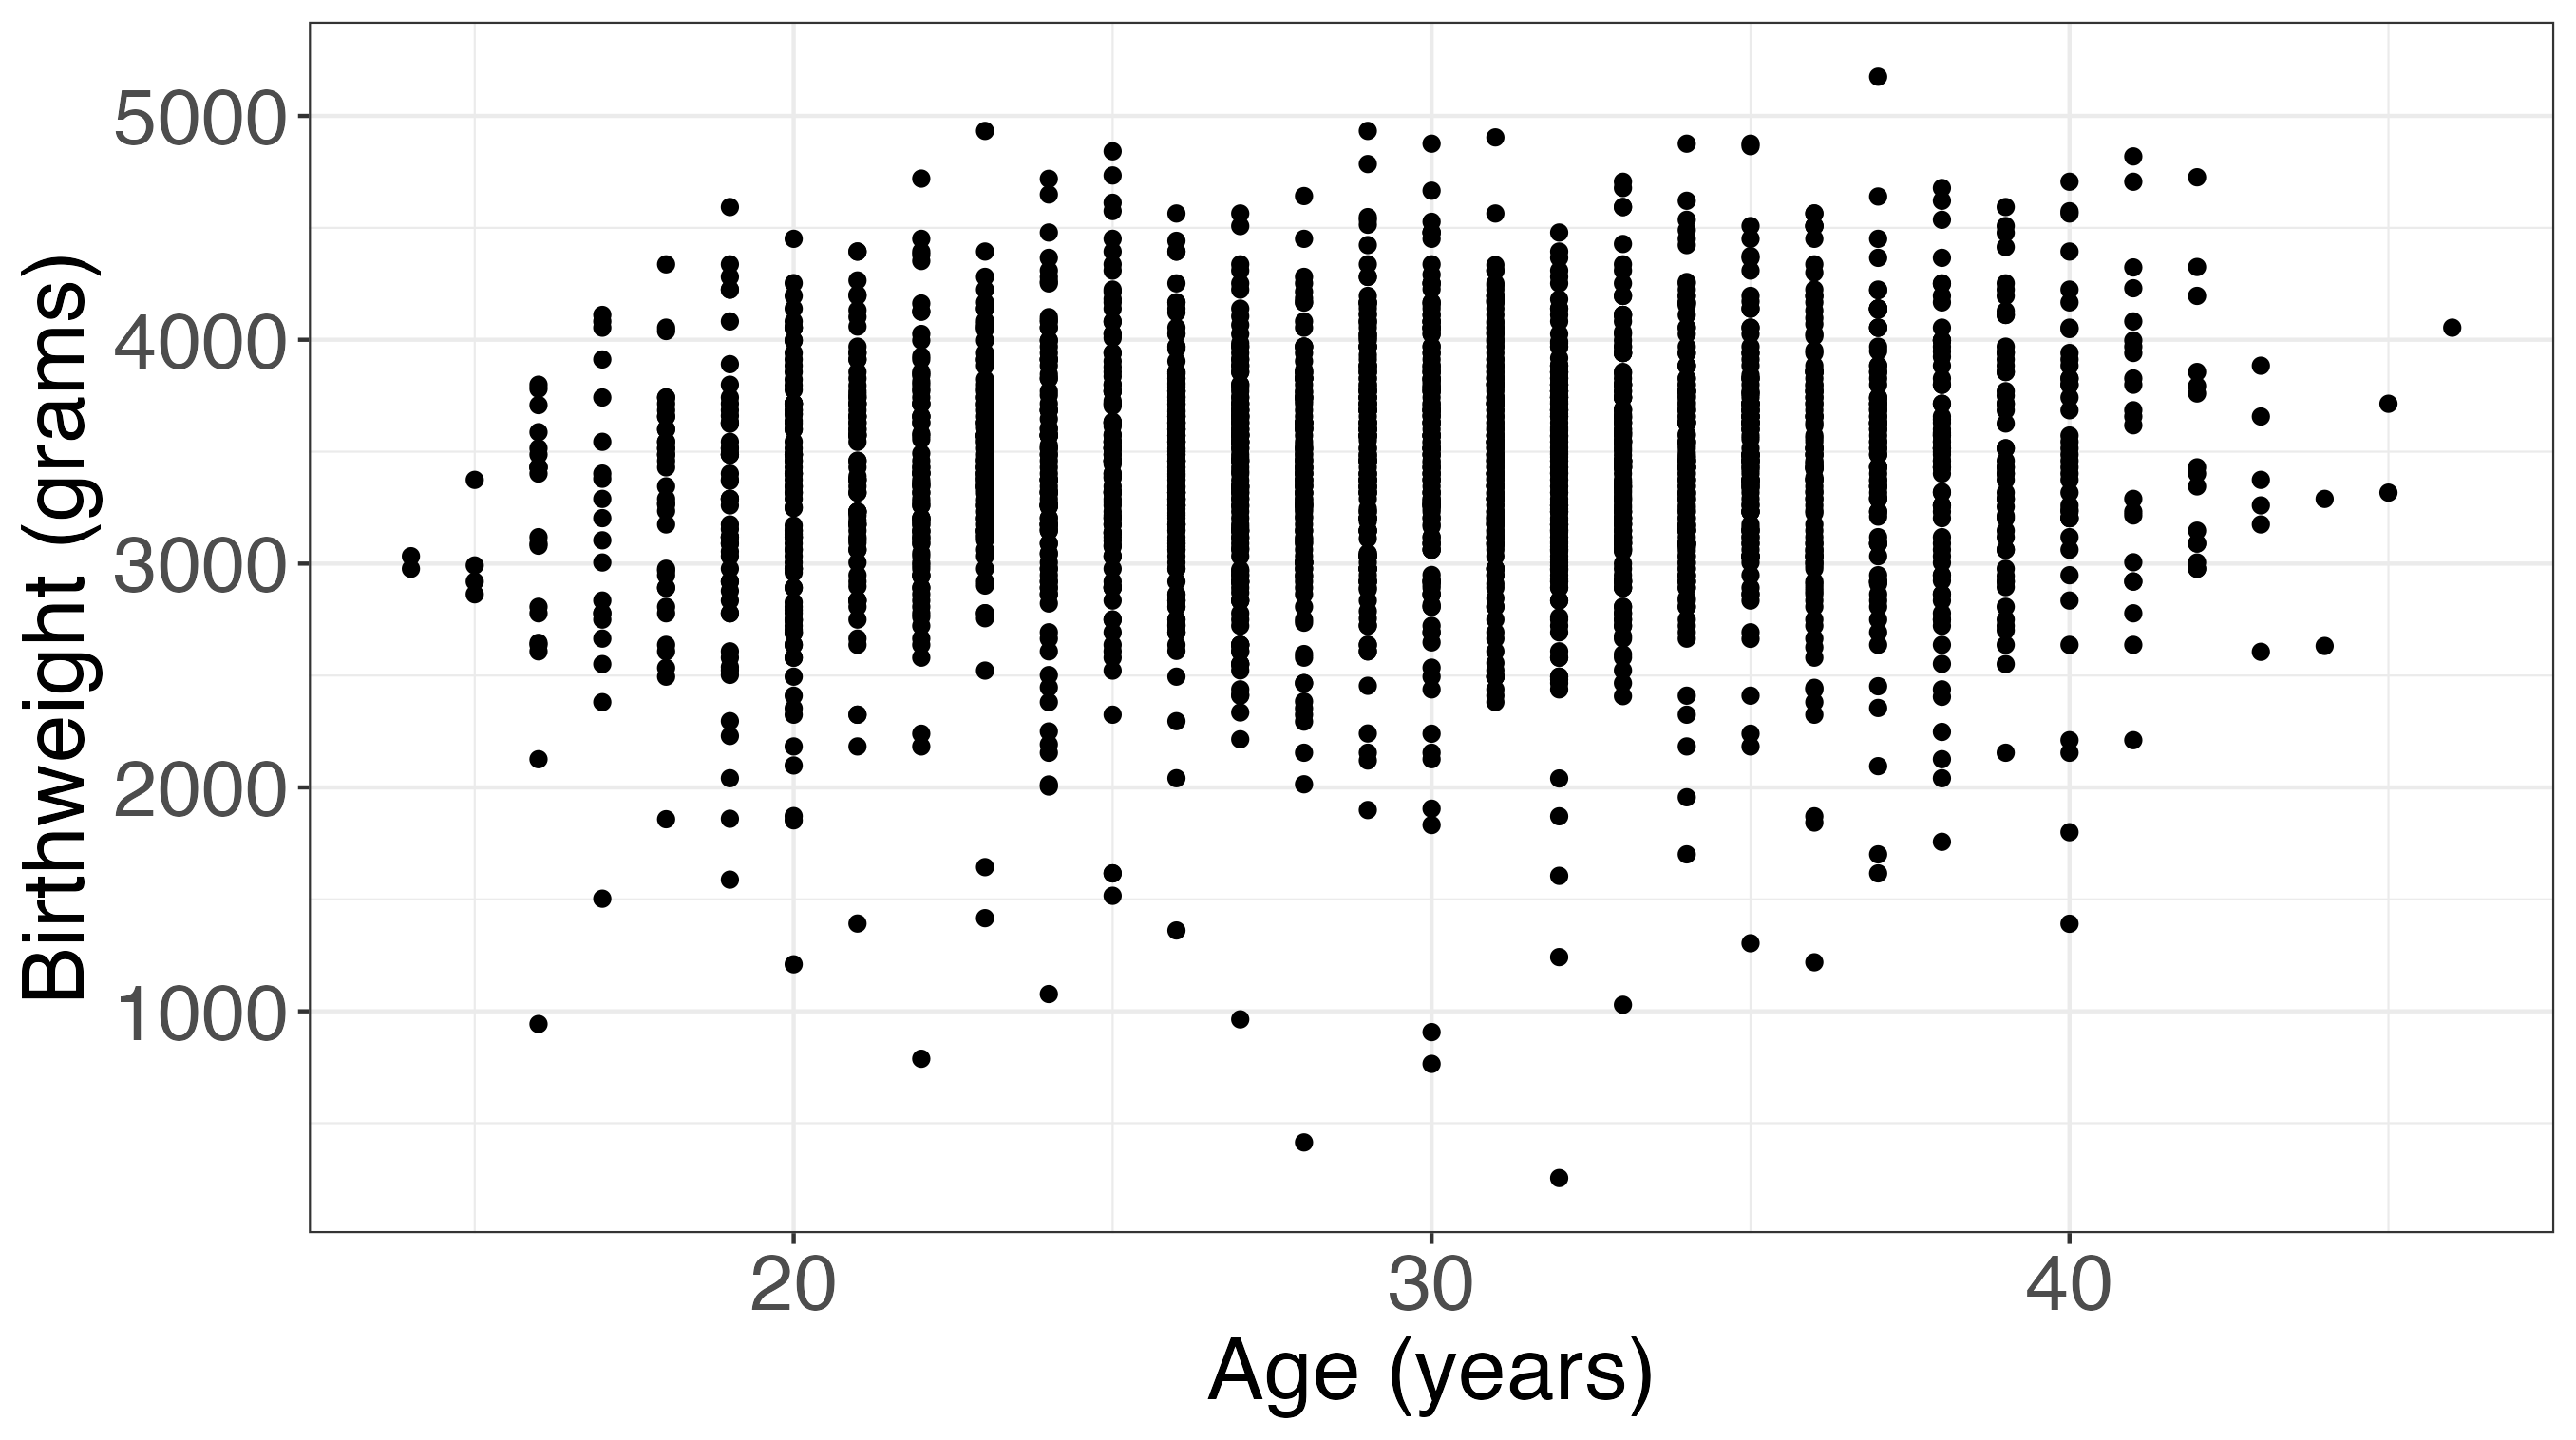
\includegraphics{fs_scatter.png}
\end{frame}

\begin{frame}{Descriptive Statistics in R}
\protect\hypertarget{descriptive-statistics-in-r}{}
This is just a small taste of the many possibilities when it comes to
tools for summarizing data.

We'll spend more time discussing descriptive statistics in Discussion
Section, including how to generate numerical summaries and graphical
summaries like these (or better ones!) in \textbackslash texttt\{R .

You'll also get practice on homework assignments and your data analysis
project!
\end{frame}

\begin{frame}{}
\protect\hypertarget{section-3}{}
Any Questions?
\end{frame}

\hypertarget{statistical-inference}{%
\section{Statistical inference}\label{statistical-inference}}

\begin{frame}{Statistical Inference}
\protect\hypertarget{statistical-inference-1}{}
Why do we do statistics?

\begin{itemize}
\item
  We can't (usually) measure everyone in our **population
\item
  *Example : all pregnant individuals in King County
\item
  Instead, we take a **sample
\item
  *Example : 2500 pregnant individuals with singleton births
\item
  Note: important to sample well so that the sample truly reflects (is
  *representative of) our population of interest
\item
  We hope that what we estimate from the sample also applies to the
  population
\item
  The process of translating from the \emph{sample to the }population is
  **statistical inference
\item
  What we estimate in the sample = \textbf{estimate or }statistic
\item
  Corresponding value in population = **parameter
\end{itemize}
\end{frame}

\begin{frame}{Statistical Inference: Work Flow}
\protect\hypertarget{statistical-inference-work-flow}{}
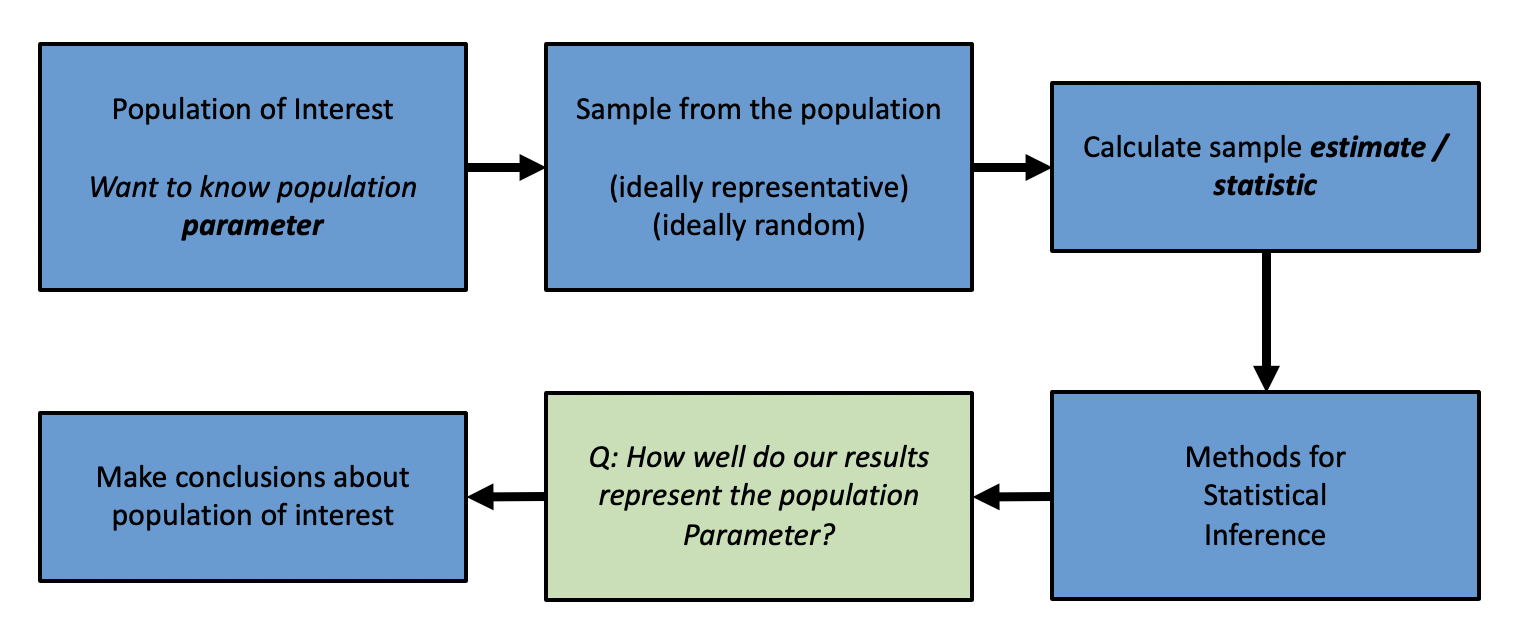
\includegraphics{statinference_workflow.png}
\end{frame}

\begin{frame}{Statistical Inference: Motivating example}
\protect\hypertarget{statistical-inference-motivating-example}{}
Consider our births dataset. We're interesting in knowing whether the
First Steps program improves birth outcomes in King County.

\begin{itemize}
\tightlist
\item
  \textbf{Scientific question}: what is the {typical} {birth outcome}
  for an individual?
\end{itemize}
\end{frame}

\begin{frame}{Statistical Inference: Motivating example}
\protect\hypertarget{statistical-inference-motivating-example-1}{}
Consider our births dataset. We're interesting in knowing whether the
First Steps program improves birth outcomes in King County.

\begin{itemize}
\tightlist
\item
  \textbf{Scientific question}: what is the {typical} {birth outcome}
  for an individual?
\item
  \textbf{Statistical question}: what is the {mean} {birth weight} for
  an individual?
\end{itemize}
\end{frame}

\begin{frame}{Statistical Inference: Motivating example}
\protect\hypertarget{statistical-inference-motivating-example-2}{}
Consider our births dataset. We're interesting in knowing whether the
First Steps program improves birth outcomes in King County.

\begin{itemize}
\tightlist
\item
  \textbf{Scientific question}: what is the {typical} {birth outcome}
  for an individual?
\item
  \textbf{Statistical question}: what is the {mean} {birth weight} for
  an individual?
\item
  \textbf{Population of interest}: all babies born in King County
\end{itemize}
\end{frame}

\begin{frame}{Statistical Inference: Motivating example}
\protect\hypertarget{statistical-inference-motivating-example-3}{}
Consider our births dataset. We're interesting in knowing whether the
First Steps program improves birth outcomes in King County.

\begin{itemize}
\tightlist
\item
  \textbf{Scientific question}: what is the {typical} {birth outcome}
  for an individual?
\item
  \textbf{Statistical question}: what is the {mean} {birth weight} for
  an individual?
\item
  \textbf{Population of interest}: all babies born in King County
\item
  \textbf{Parameter}: population mean
\end{itemize}
\end{frame}

\begin{frame}{Statistical Inference: Motivating example}
\protect\hypertarget{statistical-inference-motivating-example-4}{}
Consider our births dataset. We're interesting in knowing whether the
First Steps program improves birth outcomes in King County.

\begin{itemize}
\tightlist
\item
  \textbf{Scientific question}: what is the {typical} {birth outcome}
  for an individual?
\item
  \textbf{Statistical question}: what is the {mean} {birth weight} for
  an individual?
\item
  \textbf{Population of interest}: all babies born in King County
\item
  \textbf{Parameter}: population mean
\item
  \textbf{Sample}: 2500 singleton births in King County in 2001
\end{itemize}
\end{frame}

\begin{frame}{Statistical Inference: Motivating example}
\protect\hypertarget{statistical-inference-motivating-example-5}{}
Consider our births dataset. We're interesting in knowing whether the
First Steps program improves birth outcomes in King County.

\begin{itemize}
\item
  \textbf{Scientific question}: what is the {typical} {birth outcome}
  for an individual?
\item
  \textbf{Statistical question}: what is the {mean} {birth weight} for
  an individual?
\item
  \textbf{Population of interest}: all babies born in King County
\item
  \textbf{Parameter}: population mean
\item
  \textbf{Sample}: 2500 singleton births in King County in 2001
\item
  \textbf{Statistic/estimate}: sample mean (3414 grams)
\end{itemize}
\end{frame}

\begin{frame}{Statistical Inference: Motivating example}
\protect\hypertarget{statistical-inference-motivating-example-6}{}
Consider our births dataset. We're interesting in knowing whether the
First Steps program improves birth outcomes in King County.

\begin{itemize}
\item
  \textbf{Scientific question}: what is the {typical} {birth outcome}
  for an individual?
\item
  \textbf{Statistical question}: what is the {mean} {birth weight} for
  an individual?
\item
  \textbf{Population of interest}: all babies born in King County
\item
  \textbf{Parameter}: population mean
\item
  \textbf{Sample}: 2500 singleton births in King County in 2001
\item
  \textbf{Statistic/estimate}: sample mean (3414 grams)
\end{itemize}

\textbf{Next step}: consider what conclusions can be drawn from our
sample estimate about our population parameter. Was our sample
representative? Are there implications (statistical, ethical) to
generalizing our result to our population?
\end{frame}

\begin{frame}{Precision and Accuracy}
\protect\hypertarget{precision-and-accuracy}{}
Using descriptive statistics, we can get sample estimates

\begin{itemize}
\tightlist
\item
  e.g., the **mean birthweight for singleton births in King County in
  2001 was 3414 grams
\end{itemize}

We want to use these sample estimates to infer something about the
population

To assess how well these estimates represent the population of interest,
we need to know how \textbf{accurate and }precise they are

\begin{itemize}
\tightlist
\item
  Accuracy: are we estimating the right thing?
\item
  Precision: how variable are our estimates?
\end{itemize}

*Just like we want to describe the center and spread of variables when
we summarize our data, we also want to understand the center (accuracy)
and spread (precision) of our estimates.
\end{frame}

\begin{frame}{Precision and Accuracy}
\protect\hypertarget{precision-and-accuracy-1}{}
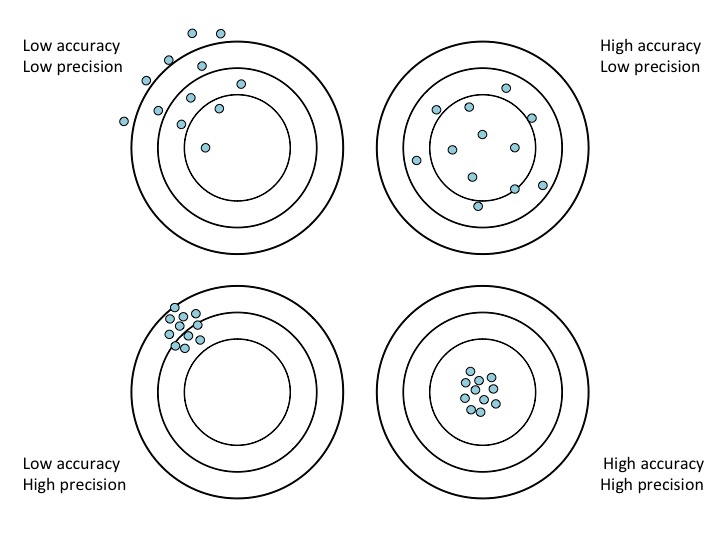
\includegraphics{accuracy.jpg}
\end{frame}

\begin{frame}{Precision, Accuracy, and Inference}
\protect\hypertarget{precision-accuracy-and-inference}{}
How do we know how precise or accurate our statistic is?

\begin{itemize}
\item
  We need to know how our statistic (estimated from a sample) would vary
  in *repeated samples
\item
  i.e., if we went out and collected another sample from this
  population, how different would the estimate be? And if we did this a
  third time, or a fourth time, or\ldots?
\item
  Our statistics are *random : the value you get will change depending
  on which sample you've ended up with
\item
  The **distribution of a random quantity describes how that random
  quantity behaves
\item
  If we know the distribution of our statistic, the center tells us
  about the (possible\({ ^1\)) accuracy and the spread tells us about
  the precision of our statistic
\end{itemize}

\small \({ ^1\) we only know how accurate our statistic is if we know
the population parameter, but we can often judge whether our statistics
are very *inaccurate based on whether our sample is representative of
the population or not
\end{frame}

\begin{frame}{Probability distributions}
\protect\hypertarget{probability-distributions}{}
The distribution of a random quantity tells you what values that
quantity can take and how likely it is to take each of those values.

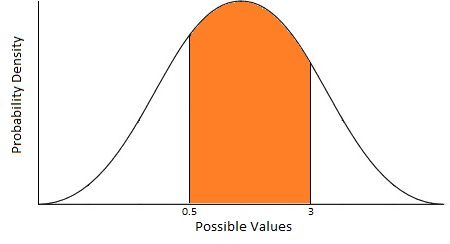
\includegraphics{Normal-density.jpg}

Figure: Area under curve = probability that our random quantity takes
values between 0.5 and 3
\end{frame}

\begin{frame}{Probability distributions: normal distribution}
\protect\hypertarget{probability-distributions-normal-distribution}{}
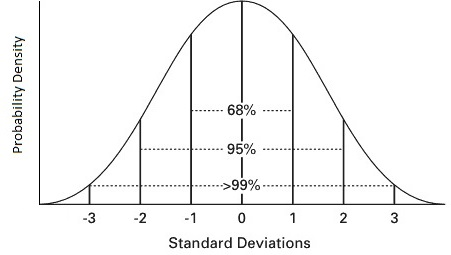
\includegraphics{Normal.jpg}

Useful property: if a random quantity is normally distributed
\((~N(\mu, \sigma^2))\), then 95 \% of the time that quantity will take
values within 1.96 standard deviations \((\sigma)\) of its mean
\((\mu)\)

\small Many of the random quantities we care about have a normal
distribution!
\end{frame}

\begin{frame}{Probability distributions: \(t\) distribution}
\protect\hypertarget{probability-distributions-t-distribution}{}
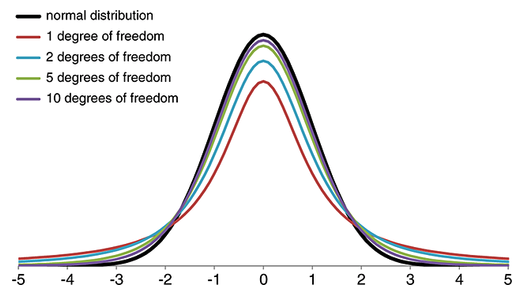
\includegraphics{tdistn.png}

The \(t\) distribution is similar to a normal distribution, but with
heavier tails. How close it is to a normal distribution depends on the
*degrees of freedom .
\end{frame}

\begin{frame}{Sampling distributions}
\protect\hypertarget{sampling-distributions}{}
**Sampling distribution : the distribution of an estimate/statistic

The Central Limit Theorem tells us the sampling distribution of some
statistics that we care about *for large samples :

\begin{itemize}
\item
  **Mean: the sampling distribution of the sample mean is approximately
  normal: \(\bar{X \sim N(\mu, \sigma^2 / n)\)
\item
  \(\mu\) = population mean
\item
  \(\sigma^2\) = population variance
\item
  \(n\) = sample size
\end{itemize}
\end{frame}

\begin{frame}{Sampling distributions}
\protect\hypertarget{sampling-distributions-1}{}
**Sampling distribution : the distribution of an estimate/statistic

The Central Limit Theorem tells us the sampling distribution of some
statistics that we care about *for large samples :

\begin{itemize}
\item
  **Mean: the sampling distribution of the sample mean is approximately
  normal: \(\bar{X \sim N(\mu, \sigma^2 / n)\)
\item
  \(\mu\) = population mean
\item
  \(\sigma^2\) = population variance
\item
  \(n\) = sample size
\item
  **Proportion: the sampling distribution of the sample proportion is
  approximately normal: \$ \textbackslash hat\{p \sim N(p, p(1-p)/n)\$
\item
  \(p\) = population proportion
\item
  \(n\) = sample size / number of trials
\end{itemize}
\end{frame}

\begin{frame}{Sampling distributions}
\protect\hypertarget{sampling-distributions-2}{}
**Sampling distribution : the distribution of an estimate/statistic

The Central Limit Theorem tells us the sampling distribution of some
statistics that we care about *for large samples :

\begin{itemize}
\item
  **Mean: the sampling distribution of the sample mean is approximately
  normal: \(\bar{X \sim N(\mu, \sigma^2 / n)\)
\item
  \(\mu\) = population mean
\item
  \(\sigma^2\) = population variance
\item
  \(n\) = sample size
\item
  **Proportion: the sampling distribution of the sample proportion is
  approximately normal: \$ \textbackslash hat\{p \sim N(p, p(1-p)/n)\$
\item
  \(p\) = population proportion
\item
  \(n\) = sample size / number of trials
\end{itemize}

Another statistic that we often care about
\$\textbackslash frac\{\bar\{X - \textbackslash mu \{s \sim t\_\{n - 1
\$

\begin{itemize}
\tightlist
\item
  \(s\) = sample standard deviation
\end{itemize}
\end{frame}

\begin{frame}{Uncertainty: Standard error}
\protect\hypertarget{uncertainty-standard-error}{}
\textbf{Sampling distribution : the distribution of an
estimate/statistic }Standard error : the standard deviation of an
estimate/statistic

Once we know the sampling distribution of our estimate, it's fairly
straightforward to figure out how *precise it is.

Example: Suppose we have to estimates. The first has sampling
distribution \(N(2, 5)\) and the second has sampling distribution
\(N(2, 1)\). *Which of these estimates is more precise?

\small (Hint: precision and variance are inversely related) \pause

\normalsize Answer: We typically describe the precision of an estimate
via its standard error. Estimates with \emph{smaller standard error are
}more precise. Therefore, the estimate with sampling distribution
\(N(2, 1)\) is more precise.
\end{frame}

\begin{frame}{Uncertainty: Standard error}
\protect\hypertarget{uncertainty-standard-error-1}{}
\textbf{Sampling distribution} : the distribution of an
estimate/statistic \textbf{Standard error} : the standard deviation of
an estimate/statistic

The sampling distribution of the sample mean \$\bar\{X\} \$ is
approximately normal: \(\bar{X } \sim N(\mu, \sigma^2/n)\)

Question : What is the standard error?

Answer : The standard deviation of the sample mean, which is
\$\sqrt{\sigma^2}/n \$.
\end{frame}

\begin{frame}{Uncertainty: Standard error}
\protect\hypertarget{uncertainty-standard-error-2}{}
\textbf{Sampling distribution} : the distribution of an
estimate/statistic \textbf{Standard error} : the standard deviation of
an estimate/statistic

The sampling distribution of the sample proportion
\$\textbackslash hat\{p \$ is approximately normal:
\(\hat{p} \sim N(p, p(1-p)/n)\)

Question : What is the standard error?

Answer : The standard deviation of the sample proportion, which is
\$\sqrt{p(1-p)}/n \$.
\end{frame}

\begin{frame}{Uncertainty: Reporting uncertainty: Motivating example}
\protect\hypertarget{uncertainty-reporting-uncertainty-motivating-example}{}
Recall our motivating example for statistical inference:

We're interesting in knowing whether the First Steps program improves
birth outcomes in King County.

\begin{itemize}
\item
  \textbf{Scientific question}: what is the typical birth outcome for an
  individual?
\item
  \textbf{Statistical question}: what is the mean birth weight for an
  individual?
\item
  \textbf{Population of interest}: all babies born in King County
\item
  \textbf{Parameter}: population mean
\item
  \textbf{Sample}: 2500 singleton births in King County in 2001
\item
  \textbf{Statistic/estimate}: sample mean (3414 grams)
\end{itemize}
\end{frame}

\begin{frame}{Reporting uncertainty: Motivating example}
\protect\hypertarget{reporting-uncertainty-motivating-example}{}
We can convert this outline into general steps for a statistical
inference procedure:

\begin{enumerate}
\item
  Start with a \textbf{scientific question}: what is the typical birth
  outcome for an individual?
\item
  Convert to a \textbf{statistical question}: what is the mean birth
  weight for an individual?
\item
  Identify the \textbf{population} (all babies born in King County) and
  \textbf{parameter} (population mean) of interest
\item
  Take a \textbf{sample} from the population: 2500 singleton births in
  King County in 2001
\end{enumerate}

Perform \textbf{statistical inference} :

\begin{enumerate}
\setcounter{enumi}{5}
\item
  Calculate the corresponding \textbf{statistic} (sample mean): 3414
  grams
\item
  Quantify the \textbf{uncertainty} in your statistic
\item
  \textbf{Make conclusions} about your original scientific and
  statistical questions
\end{enumerate}
\end{frame}

\begin{frame}{Reporting uncertainty: Motivating example}
\protect\hypertarget{reporting-uncertainty-motivating-example-1}{}
We can convert this outline into general steps for a statistical
inference procedure:

\begin{enumerate}
\item
  Start with a \textbf{scientific question}: what is the typical birth
  outcome for an individual?
\item
  Convert to a \textbf{statistical question}: what is the mean birth
  weight for an individual?
\item
  Identify the \textbf{population} (all babies born in King County) and
  \textbf{parameter} (population mean) of interest
\item
  Take a \textbf{sample} from the population: 2500 singleton births in
  King County in 2001
\end{enumerate}

Perform \textbf{statistical inference} :

\begin{enumerate}
\setcounter{enumi}{5}
\tightlist
\item
  Calculate the corresponding \textbf{statistic} (sample mean): 3414
  grams
\item
  Quantify the \textbf{uncertainty} in your statistic\(\leftarrow\)
  \textbf{two options}
\end{enumerate}

\begin{itemize}
\tightlist
\item
  Make conclusions about your original scientific and statistical
  questions
\end{itemize}
\end{frame}

\begin{frame}{Reporting uncertainty: Motivating example}
\protect\hypertarget{reporting-uncertainty-motivating-example-2}{}
We've calculated our statistic: average birthweight = 3414 grams

Now we need to quantify our uncertainty in this estimate.

{Option 1}: use the standard error

We estimate that the average birthweight is 3414 grams, with standard
error 0.224.

{Option 2}: use a 95 \% confidence interval (est \(\pm 1.96 \times SE\))

We estimate that the average birthweight is 3414 grams. Based on a 95 \%
confidence interval, this observed average would not be considered
unusual if the true average birthweight were between 3413.6 and 3414.5
grams.
\end{frame}

\begin{frame}{Confidence Intervals}
\protect\hypertarget{confidence-intervals}{}
What does a 95 \% confidence interval really mean, and how do we
correctly interpret it?

The procedure of creating a 95 \% confidence interval (est
\(\pm 1.96 \times SE\)) gives us a range of values based on our sample.

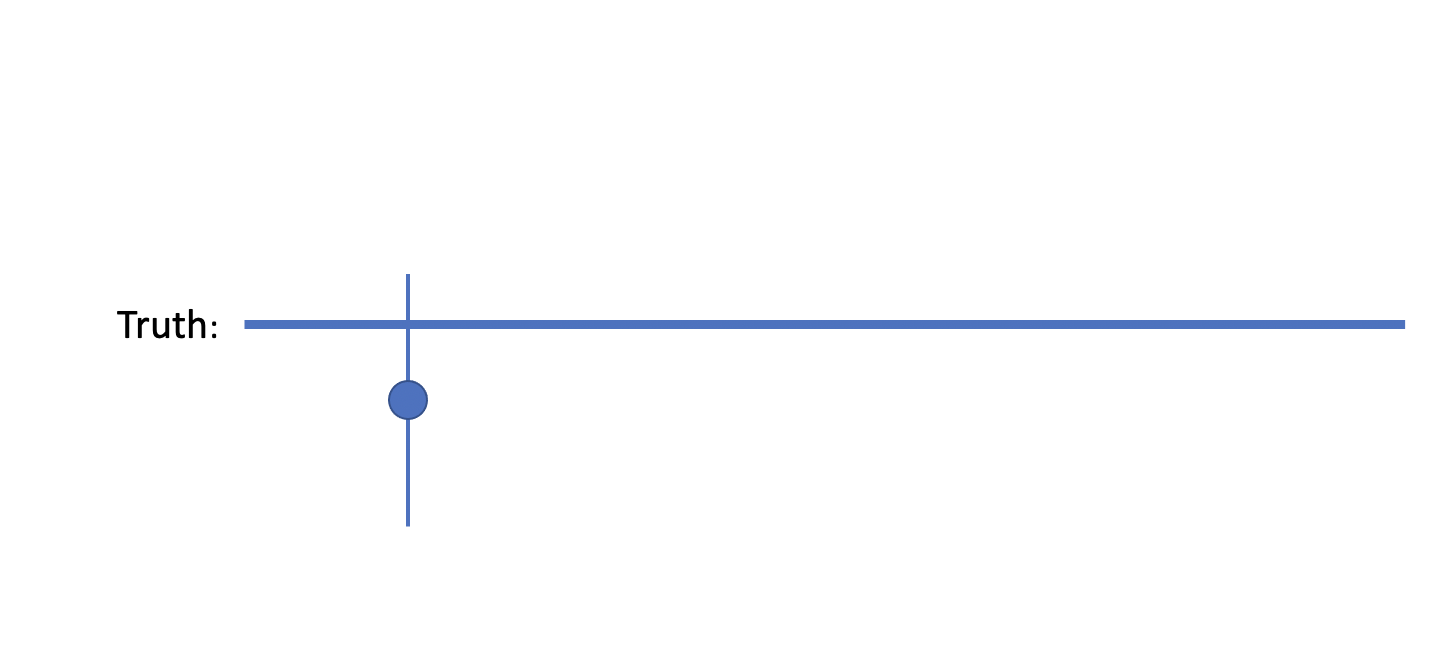
\includegraphics{ci1.png}
\end{frame}

\begin{frame}{Confidence Intervals}
\protect\hypertarget{confidence-intervals-1}{}
What does a 95 \% confidence interval really mean, and how do we
correctly interpret it?

The procedure of creating a 95 \% confidence interval (est
\(\pm 1.96 \times SE\)) gives us a range of values based on our sample.

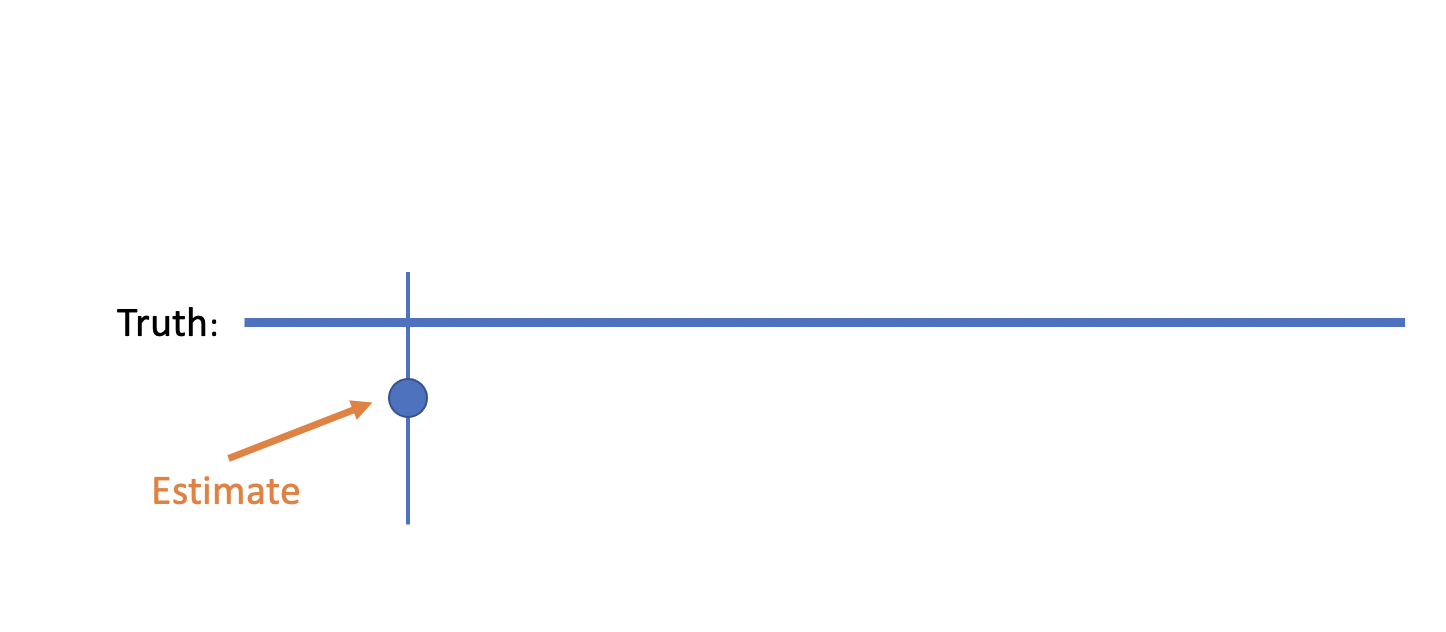
\includegraphics{ci2.png}
\end{frame}

\begin{frame}{Confidence Intervals}
\protect\hypertarget{confidence-intervals-2}{}
What does a 95 \% confidence interval really mean, and how do we
correctly interpret it?

The procedure of creating a 95 \% confidence interval (est
\(\pm 1.96 \times SE\)) gives us a range of values based on our sample.

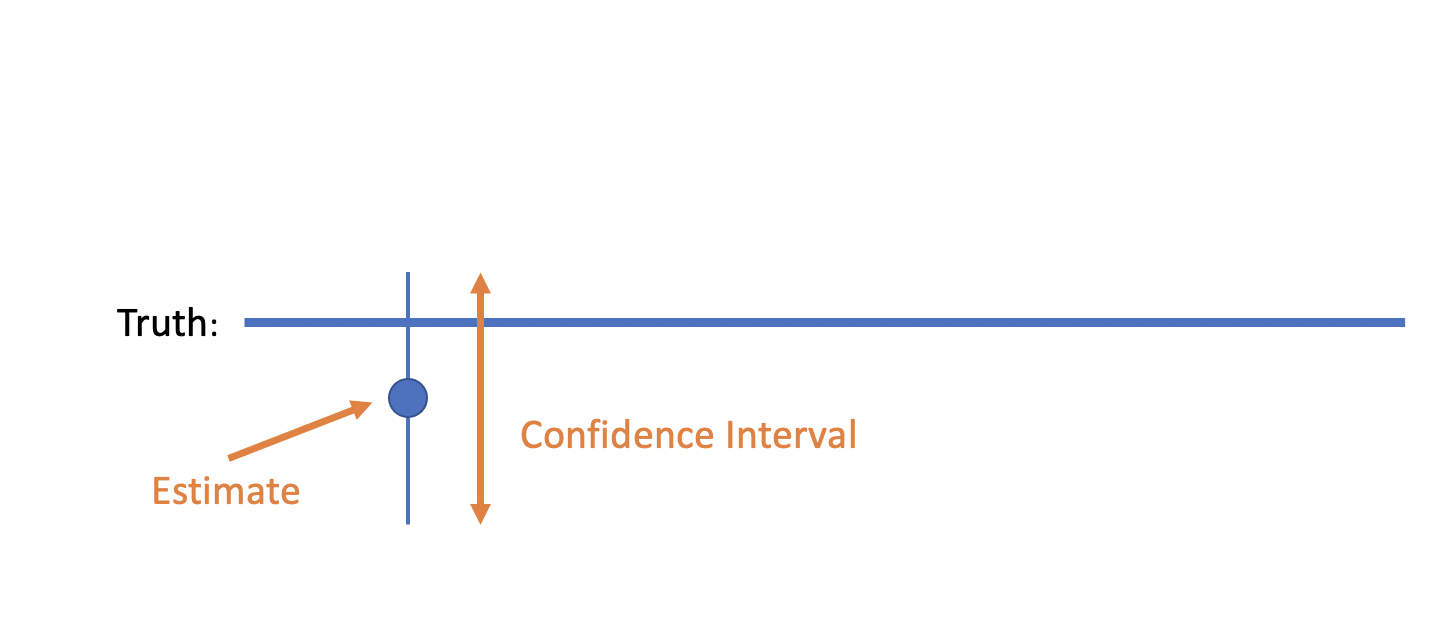
\includegraphics{ci3.png}
\end{frame}

\begin{frame}{Confidence Intervals}
\protect\hypertarget{confidence-intervals-3}{}
The particular range of values that we get depends on the sample data,
and will change if we go collect a second sample \ldots{}

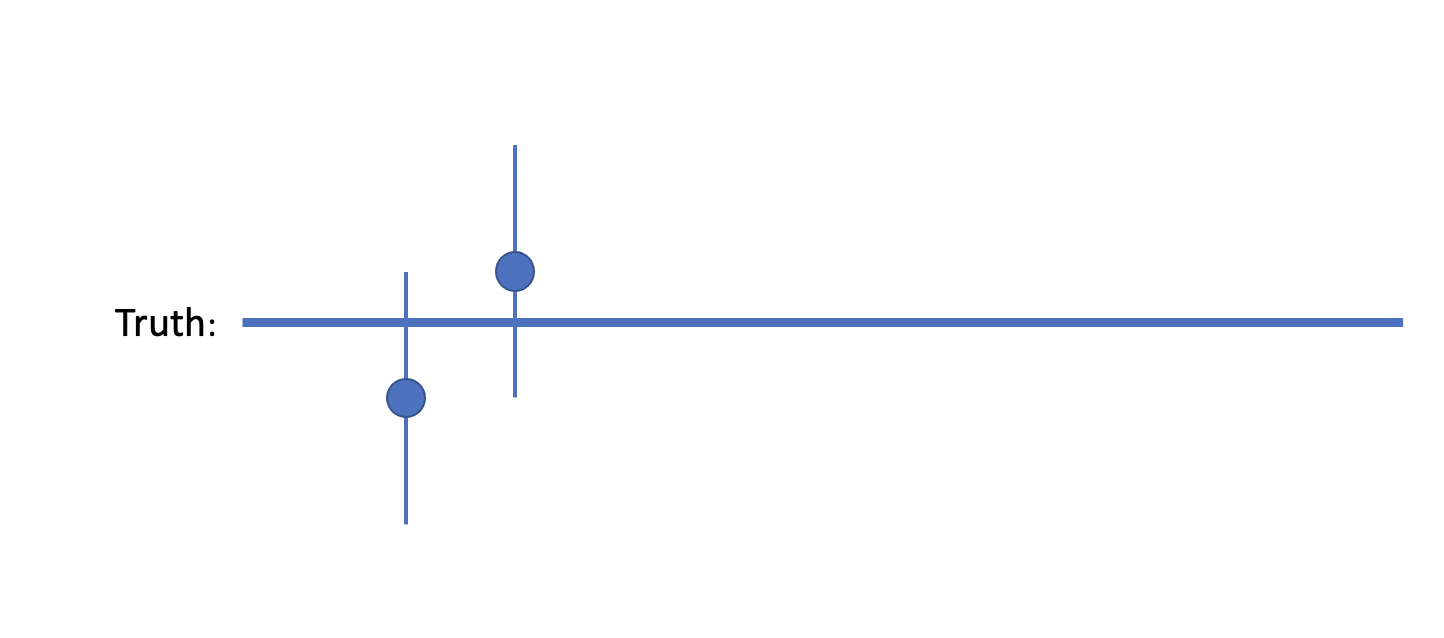
\includegraphics{ci4.png}
\end{frame}

\begin{frame}{Confidence Intervals}
\protect\hypertarget{confidence-intervals-4}{}
\ldots{} or a third sample \ldots{}

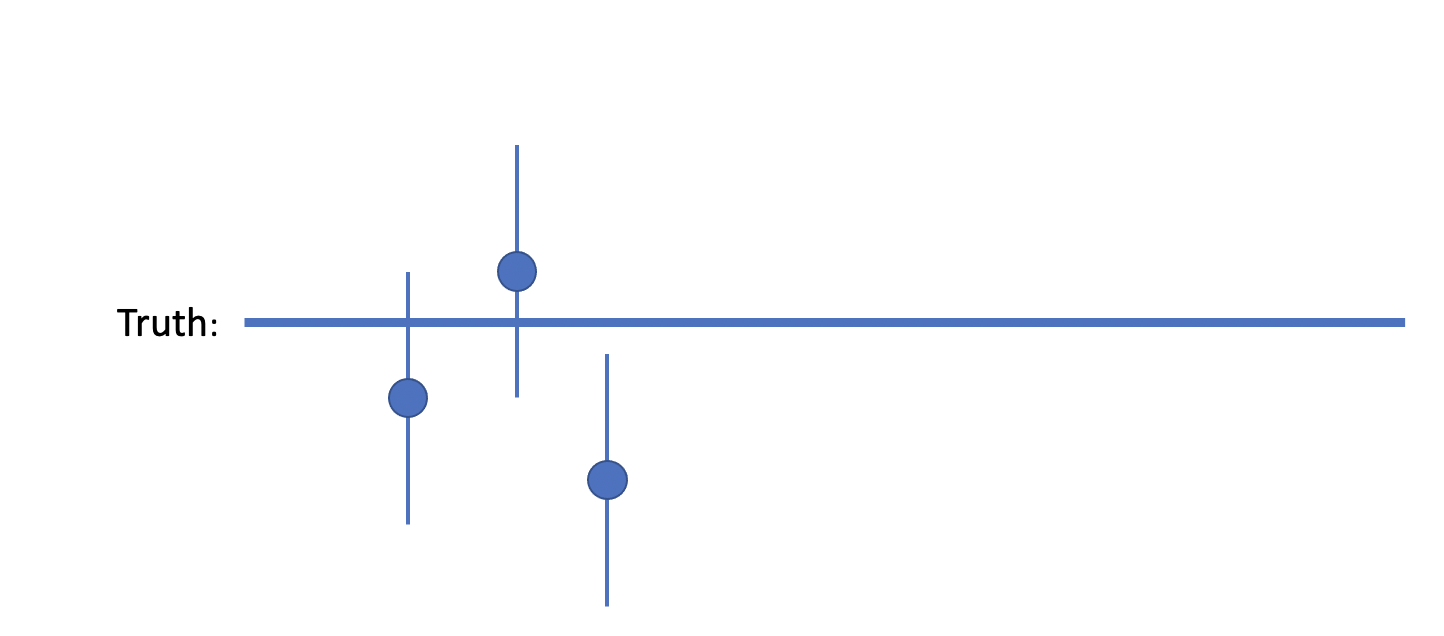
\includegraphics{ci5.png}
\end{frame}

\begin{frame}{Confidence Intervals}
\protect\hypertarget{confidence-intervals-5}{}
Over (hypothetical) \textbf{repeated sampling , 95 \% }of these
intervals will cover the truth.

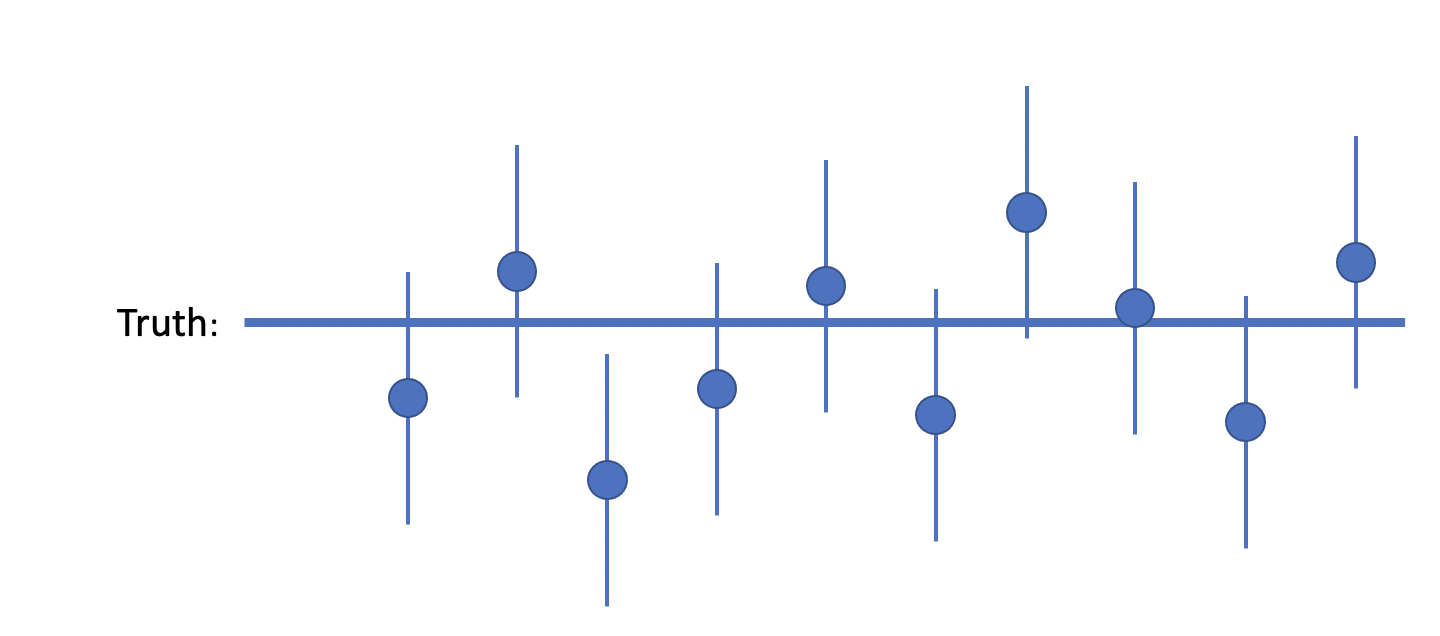
\includegraphics{ci6.png}
\end{frame}

\begin{frame}{Confidence Intervals}
\protect\hypertarget{confidence-intervals-6}{}
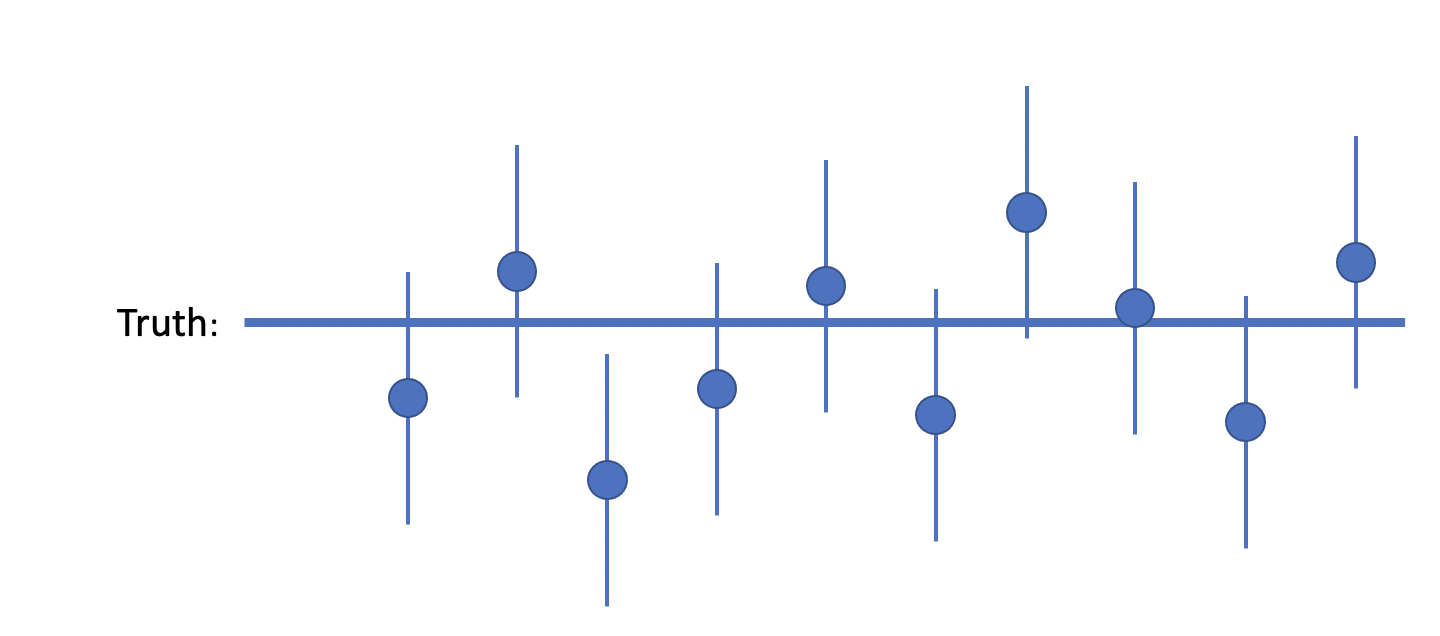
\includegraphics{ci6.png}

Important: it is not \textbf{our interval} that contains the truth 95 \%
of the time. Our interval either contains the truth, or it doesn't (as
the image above shows). It is the \textbf{procedure} of computing
confidence intervals over \textbf{repeated sampling} that gives us 95 \%
coverage of the truth.
\end{frame}

\begin{frame}{Interpreting Confidence Intervals: Example}
\protect\hypertarget{interpreting-confidence-intervals-example}{}
95 \% CI for mean birthweight in grams is: (3413.6, 3414.5)

Which of these is the correct interpretation?

\textbackslash begin\{enumerate - 95 \% of children have birthweights
between 3413.6 and 3414.5 grams. - Our observed sample mean of 3414
grams would not be considered unusual if the true population mean
birthweight were between 3413.6 and 3414.5 grams. - There is a 95 \%
chance that the true population mean birthweight is between 3413.6 and
3414.5 grams.
\end{frame}

\begin{frame}{Interpreting Confidence Intervals: Example}
\protect\hypertarget{interpreting-confidence-intervals-example-1}{}
95 \% CI for mean birthweight in grams is: (3413.6, 3414.5)

Which of these is the correct interpretation?

\textbackslash begin\{enumerate - 95 \% of children have birthweights
between 3413.6 and 3414.5 grams. - {Our} observed sample mean of 3414
grams would not be considered unusual if the true population mean
birthweight were between 3413.6 and 3414.5 grams. - There is a 95 \%
chance that the true population mean birthweight is between 3413.6 and
3414.5 grams.*

\emph{this} is a common mistake, and is \emph{not} the correct
interpretation of a confidence interval!
\end{frame}

\begin{frame}{Interpreting Confidence Intervals: How-to}
\protect\hypertarget{interpreting-confidence-intervals-how-to}{}
Confidence intervals should always be interpreted \textbf{in context} .

When interpreting confidence intervals, it may be useful to have a
``word formula'' to refer back to. An example of this is:

Our observed sample estimate of \_\_\_ \textless span units would not be
considered unusual if the true population were between \_\_\_ and \_\_\_
.
\end{frame}

\begin{frame}{Interpreting Confidence Intervals: How-to}
\protect\hypertarget{interpreting-confidence-intervals-how-to-1}{}
Confidence intervals should always be interpreted *in context .

When interpreting confidence intervals, it may be useful to have a
``word formula'' to refer back to. An example of this is:

Our observed sample estimate of \_\_\_ units would not be considered
unusual if the true population parameter were between \_\_\_ and \_\_\_
units .

Replacing the words and filling in the blanks for our example, we get:

Our observed sample mean of 3414 grams would not be considered unusual
if the true population mean birthweight were between 3413.6 and 3414.5 .
\end{frame}

\begin{frame}{Statistical Inference: New Example}
\protect\hypertarget{statistical-inference-new-example}{}
\begin{enumerate}
\tightlist
\item
  \textbf{Scientific question}: do birth parents in King County who
  participated in First Steps (FS) have {different } {birth outcomes} ?
\end{enumerate}
\end{frame}

\begin{frame}{Statistical Inference: New Example}
\protect\hypertarget{statistical-inference-new-example-1}{}
\begin{enumerate}
\tightlist
\item
  \textbf{Scientific question}: do birth parents in King County who
  participated in First Steps (FS) have {different }{birth outcomes} ?
\item
  \textbf{Statistical question}: is there a {difference in average}
  {birthweight} between birth parents in FS and those not in the
  program?
\end{enumerate}
\end{frame}

\begin{frame}{Statistical Inference: New Example}
\protect\hypertarget{statistical-inference-new-example-2}{}
\begin{enumerate}
\tightlist
\item
  \textbf{Scientific question}: do birth parents in King County who
  participated in First Steps (FS) have {different }{birth outcomes} ?
\item
  \textbf{Statistical question}: is there a {difference in average}
  {birthweight} between birth parents in FS and those not in the
  program?
\item
  \textbf{Population} = all babies born in King County,
  \textbf{parameter} = difference in population means (between babies
  born to parents in FS vs.~not)
\end{enumerate}
\end{frame}

\begin{frame}{Statistical Inference: New Example}
\protect\hypertarget{statistical-inference-new-example-3}{}
\begin{enumerate}
\tightlist
\item
  \textbf{Scientific question}: do birth parents in King County who
  participated in First Steps (FS) have {different }{birth outcomes} ?
\item
  \textbf{Statistical question}: is there a {difference in average}
  {birthweight} between birth parents in FS and those not in the
  program?
\item
  \textbf{Population} = all babies born in King County,
  \textbf{parameter} = difference in population means (between babies
  born to parents in FS vs.~not)
\item
  Take a \textbf{sample} from the population: 2500 singleton births in
  King County in 2001
\end{enumerate}
\end{frame}

\begin{frame}{Statistical Inference: New Example}
\protect\hypertarget{statistical-inference-new-example-4}{}
\begin{enumerate}
\item
  \textbf{Scientific question}: do birth parents in King County who
  participated in First Steps (FS) have {different }{birth outcomes} ?
\item
  \textbf{Statistical question}: is there a {difference in average}
  {birthweight} between birth parents in FS and those not in the
  program?
\item
  \textbf{Population} = all babies born in King County,
  \textbf{parameter} = difference in population means (between babies
  born to parents in FS vs.~not)
\item
  Take a \textbf{sample} from the population: 2500 singleton births in
  King County in 2001
\item
  Perform \textbf{statistical inference} :

  \begin{enumerate}
  [i.]
  \tightlist
  \item
    Calculate the corresponding \textbf{statistic} (difference in sample
    means between FS vs.~not)
  \item
    Quantify the uncertainty in our statistic
  \item
    Perform a hypothesis test
  \end{enumerate}
\end{enumerate}
\end{frame}

\begin{frame}{Statistical Inference: New Example}
\protect\hypertarget{statistical-inference-new-example-5}{}
\begin{enumerate}
\item
  \textbf{Scientific question}: do birth parents in King County who
  participated in First Steps (FS) have {different }{birth outcomes} ?
\item
  \textbf{Statistical question}: is there a {difference in average}
  {birthweight} between birth parents in FS and those not in the
  program?
\item
  \textbf{Population} = all babies born in King County,
  \textbf{parameter} = difference in population means (between babies
  born to parents in FS vs.~not)
\item
  Take a \textbf{sample} from the population: 2500 singleton births in
  King County in 2001
\item
  Perform \textbf{statistical inference} :

  \begin{enumerate}
  [i.]
  \tightlist
  \item
    Calculate the corresponding \textbf{statistic} (difference in sample
    means between FS vs.~not)
  \item
    Quantify the uncertainty in our statistic
  \item
    Perform a hypothesis test
  \end{enumerate}
\item
  Make conclusions in context of original questions
\end{enumerate}
\end{frame}

\begin{frame}{Statistical Inference: New Example}
\protect\hypertarget{statistical-inference-new-example-6}{}
To perform statistical inference, we need:

A \textbf{statistic} : difference in average birthweight \textbf{in our
sample} between babies born to parents in FS vs.~not in FS

\textbf{Uncertainty} in our statistic: 95 \% confidence interval for
difference in average birthweight

To perform a \textbf{hypothesis test}:

\begin{itemize}
\item
  \textbf{Null and alternative hypotheses} :

  \begin{itemize}
  \tightlist
  \item
    \(H_0\): \(\mu_{\text{FS}} - \mu_{\text{no FS}} = 0\)
  \item
    \(H_1\): \(\mu_{\text{FS}} - \mu_{\text{no FS}} \neq 0\)
  \end{itemize}
\item
  \textbf{Choice of test} : two-sample t-test (unequal variance)

  \begin{itemize}
  \tightlist
  \item
    Test if the averages in two independent groups are equal
  \item
    We will not assume variance in birthweight is the same in babies
    born to parents in FS vs.~not in FS
  \end{itemize}
\end{itemize}
\end{frame}

\begin{frame}{Statistical Inference: New Example}
\protect\hypertarget{statistical-inference-new-example-7}{}
We can conduct a two-sample t-test to answer this question in \texttt{R}
:

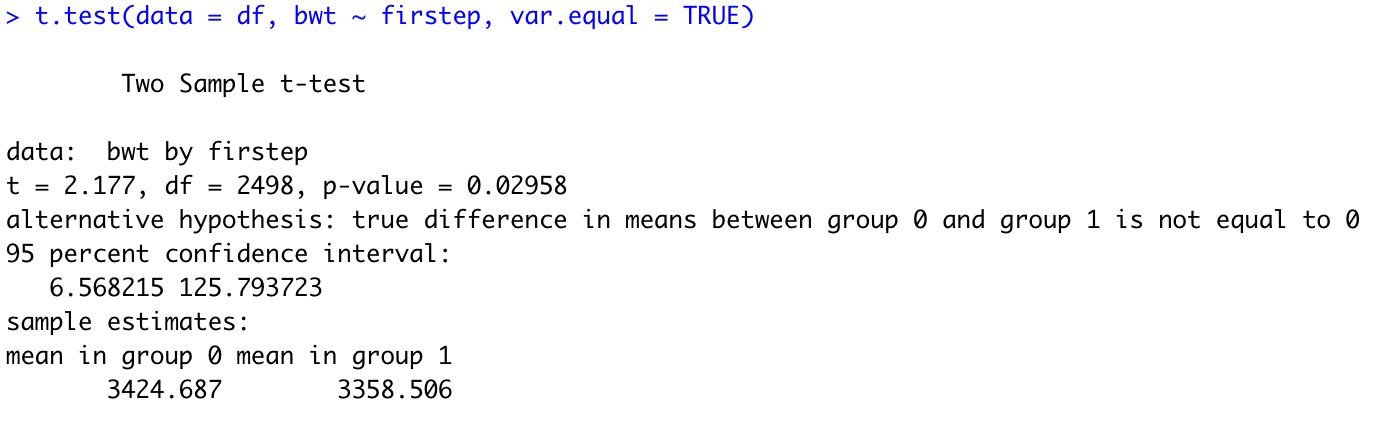
\includegraphics{ttest1.png}
\end{frame}

\begin{frame}{Statistical Inference: New Example}
\protect\hypertarget{statistical-inference-new-example-8}{}
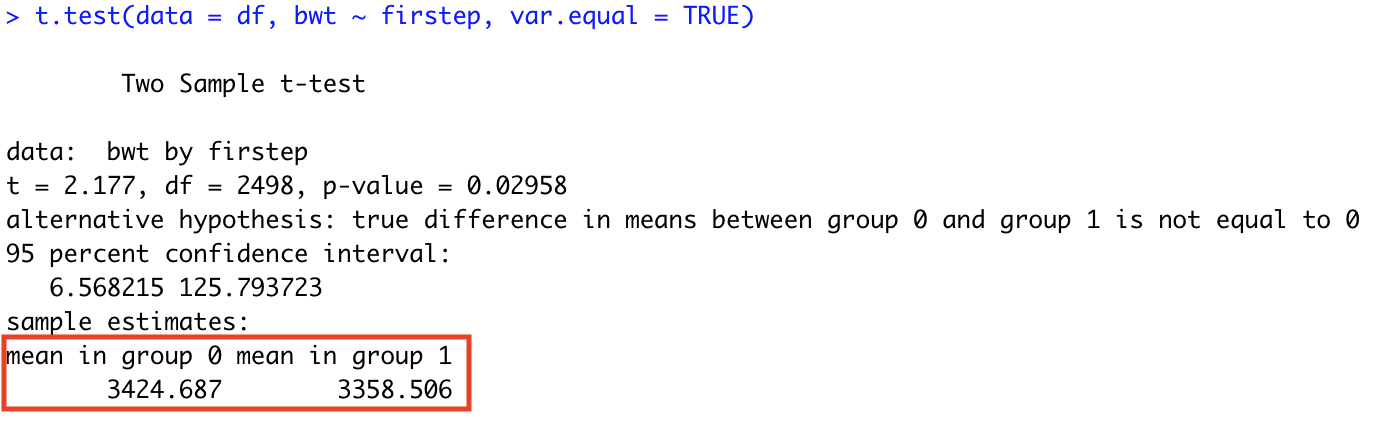
\includegraphics{ttest2.png}

\begin{itemize}
\tightlist
\item
  The observed difference in means is \(3424.687- 3358.506 \approx 66\)
  grams, with group \(0\) having the higher mean
\end{itemize}
\end{frame}

\begin{frame}{Statistical Inference: New Example}
\protect\hypertarget{statistical-inference-new-example-9}{}
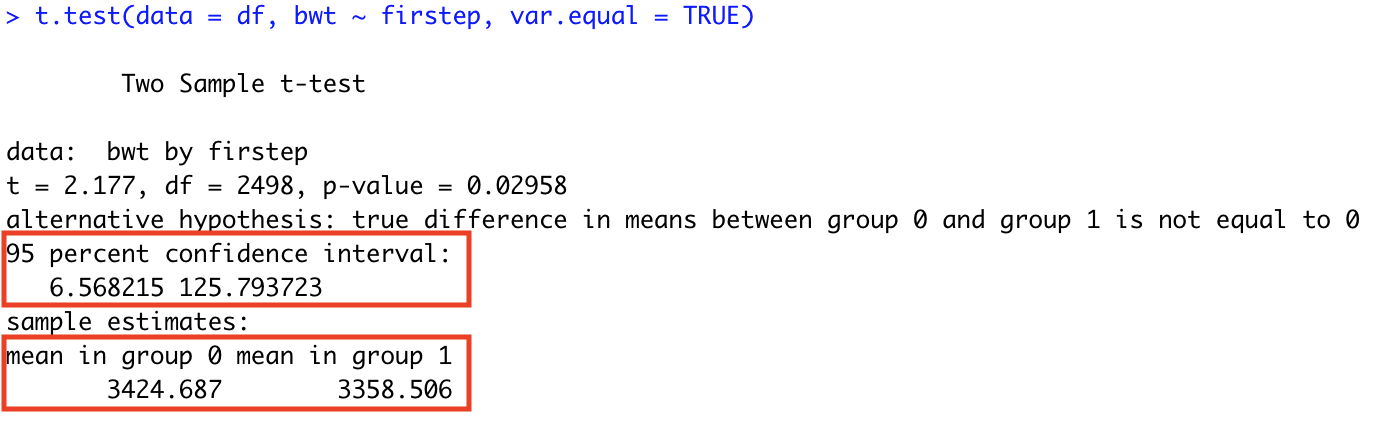
\includegraphics{ttest3.png}

\begin{itemize}
\tightlist
\item
  The observed difference in means is \(3424.687- 3358.506 \approx 66\)
  grams, with group \(0\) having the higher mean
\item
  The 95 \% confidence interval for the difference in means is
  \((6.57, 125.79)\)
\end{itemize}
\end{frame}

\begin{frame}{Statistical Inference: New Example}
\protect\hypertarget{statistical-inference-new-example-10}{}
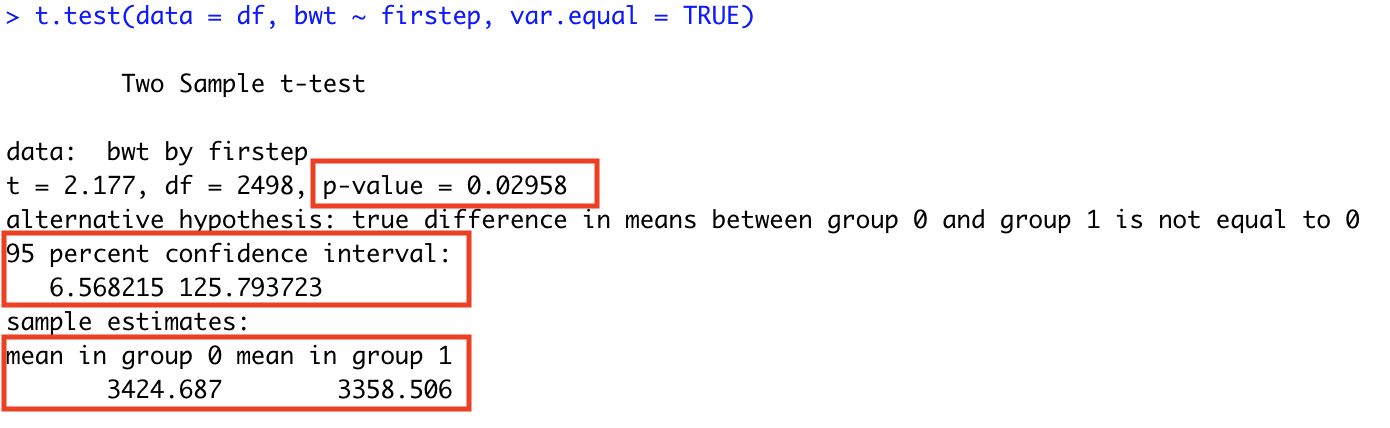
\includegraphics{ttest4.png}

\begin{itemize}
\tightlist
\item
  The observed difference in means is \(3424.687- 3358.506 \approx 66\)
  grams, with group \(0\) having the higher mean
\item
  The 95 \% confidence interval for the difference in means is
  \((6.57, 125.79)\)
\item
  The p-value corresponding to this test is \(0.03\)
\end{itemize}
\end{frame}

\begin{frame}{Interpreting p-values}
\protect\hypertarget{interpreting-p-values}{}
**Definition: a \emph{p-value is the probability of obtaining a test
statistic }as or more extreme than the observed test statistic (computed
from your data) under the null hypothesis

\begin{itemize}
\tightlist
\item
  {[}{]} \textbackslash textcolor\{red \{Not the probability that the
  alternative hypothesis is true!
\end{itemize}

(A less official definition): a *p-value is a number between 0 and 1
that quantifies the statistical strength of your evidence against the
null hypothesis

Values closer to 0 correspond to stronger evidence

\begin{itemize}
\tightlist
\item
  Reject \(H_0\) if p-value (\(p\)) is smaller than some pre-specified
  threshold \(\alpha\) (usually 0.05)
\item
  If \(p < \alpha\) we declare''statistical significance'' and reject
  \(H_0\)
\item
  {We never accept the null hypothesis}: our options are to ``reject
  \(H_0\)'' or ``fail to reject \(H_0\)''
\end{itemize}
\end{frame}

\begin{frame}{Statistical Inference: New Example}
\protect\hypertarget{statistical-inference-new-example-11}{}
Interpreting our results:

\begin{itemize}
\tightlist
\item
  *Statistic: We estimate that the difference in mean birthweight
  between babies born to birth parents in FS vs.~those not in FS is 66
  grams (with those not in FS having higher mean birthweight).
\end{itemize}
\end{frame}

\begin{frame}{Statistical Inference: New Example}
\protect\hypertarget{statistical-inference-new-example-12}{}
Interpreting our results:

\begin{itemize}
\tightlist
\item
  *Statistic: We estimate that the difference in mean birthweight
  between babies born to birth parents in FS vs.~those not in FS is 66
  grams (with those not in FS having higher mean birthweight).
\item
  *Uncertainty: Based on a 95 \% confidence interval, this observed
  difference would not be surprising if the true difference were between
  6.57 and 125.79 grams.
\end{itemize}
\end{frame}

\begin{frame}{Statistical Inference: New Example}
\protect\hypertarget{statistical-inference-new-example-13}{}
Interpreting our results:

\begin{itemize}
\tightlist
\item
  *Statistic: We estimate that the difference in mean birthweight
  between babies born to birth parents in FS vs.~those not in FS is 66
  grams (with those not in FS having higher mean birthweight).
\item
  *Uncertainty: Based on a 95 \% confidence interval, this observed
  difference would not be surprising if the true difference were between
  6.57 and 125.79 grams.
\item
  *Hypothesis test p-value: These data provide statistically significant
  evidence that the difference in mean birthweight between groups is
  different from zero (\(p < 0.05\)).
\end{itemize}
\end{frame}

\begin{frame}{Statistical Inference: New Example}
\protect\hypertarget{statistical-inference-new-example-14}{}
Interpreting our results:

\begin{itemize}
\tightlist
\item
  *Statistic: We estimate that the difference in mean birthweight
  between babies born to birth parents in FS vs.~those not in FS is 66
  grams (with those not in FS having higher mean birthweight).
\item
  *Uncertainty: Based on a 95 \% confidence interval, this observed
  difference would not be surprising if the true difference were between
  6.57 and 125.79 grams.
\item
  *Hypothesis test p-value: These data provide statistically significant
  evidence that the difference in mean birthweight between groups is
  different from zero (\(p < 0.05\)).
\item
  *Conclusion: These data provide statistically significant evidence to
  suggest that First Steps participation is associated with birthweight
  in children.
\end{itemize}
\end{frame}

\begin{frame}{Statistical Inference: New Example}
\protect\hypertarget{statistical-inference-new-example-15}{}
Interpreting our results:

\begin{itemize}
\tightlist
\item
  *Statistic: We estimate that the difference in mean birthweight
  between babies born to birth parents in FS vs.~those not in FS is 66
  grams (with those not in FS having higher mean birthweight).
\item
  *Uncertainty: Based on a 95 \% confidence interval, this observed
  difference would not be surprising if the true difference were between
  6.57 and 125.79 grams.
\item
  *Hypothesis test p-value: These data provide statistically significant
  evidence that the difference in mean birthweight between groups is
  different from zero (\(p < 0.05\)).
\item
  *Conclusion: These data provide statistically significant evidence to
  suggest that First Steps participation is associated with birthweight
  in children.
\end{itemize}

Always give 4 numbers: point estimate, confidence interval (lower,
upper), p-value (even when not significant!)

\#\#

Any Questions?
\end{frame}

\end{document}
